%\documentclass[12pt] {newrucsthesis}    % changed default font to 12pt
\documentclass[12pt] {newrucsthesis}    % changed default font to 12pt

	% preamble stuff here
\usepackage{graphicx}  % need this for figures etc.
\usepackage{url}  % to handle urls 
\usepackage{booktabs}
\usepackage[comma,authoryear]{natbib}    %  includes \citet (textual), and \citep (parenthesized) -- can be used with numbered styles too
%% include any other packages that you need for your thesis  ....

\renewcommand {\cite} {\citep}  % default for cite is citet in natbib - so change it
\newcommand {\shortcite} {\citeyearpar}  % for date only citations
\renewcommand{\floatpagefraction}{.9}
\providecommand{\tightlist}{%
\setlength{\itemsep}{0pt}\setlength{\parskip}{0pt}}

\expandafter\def\expandafter\quote\expandafter{\quote\small\singlespacing}


% \renewcommand\bibname{References}    % if not using newrucsthesis sty file


\begin{document}

   
\title{ Novel Approaches to Authorship Attribution}
\author{ Gareth Terence Bryant Dwyer }
\date { July 2017 }
\maketitle  

\acm
I hereby confirm that the thesis presented here is my own work, with all assistance acknowledged.
\\
\\
\\
\\
\\
Gareth Dwyer

Groningen, September 2017
\\
\\
\\
A thesis submitted in fulfillment of the requirements for the degree of Master of Science in Language and Communication Technologies
\\
\\




\abstract
Authorship Attribution is the study of identifying people by their writing style. We present several approaches to achieving this goal, looking at both Authorship Identification problems (in which we attempt to predict which of a limited set of candidate authors wrote a disputed text) and Authorship Verification problems (in which we attempt to predict whether or not two texts are written by the same author). We test and compare several techniques, including an unsupervised method that relies on descriptive statistics; methods which use Support Vector Machines; and methods which use Neural Networks. We compare our methods to previous state of the art results and present results on a new large dataset, built from Yelp reviews, which we introduce. Although in many cases our methods failed to beat previous state of the art results, we show that all three broad techniques are viable strategies for Authorship Attribution tasks, and we discuss the advantages and disadvantages of each approach.

\ack
Moving from a small town in South Africa to Europe was quite an adventure for me, and I have met so many wonderful, kind, and thought-provoking people along the road. Each of them have contributed in some small way to teaching me New Things, many of which are represented somehow in this work. I asked if I could publish all their names here, but apparently that's a no-no (even in size six font), so I'm picking a few of them at random and hoping that the others never read this.

Thank you Dietrich for providing advice from afar.

Thank you Malvina for all the guidance and help, and for changing my ideas about what Academia is. And for that ten minute talk about Authorship Attribution that led to this work.

Thank you Esther for the shared ideas and long discussions. Working through difficult problems together made them so much more enjoyable than fighting them alone. You helped me adjust when everything was new.

Thank you Masha for your company, for sharing your home, food and drink, and many hours of laughter and commiseration. I hope we can spend many more hours together in the future without deadlines hanging over our heads.

Thank you Roman for helping out with understanding scary theoretical concepts from the moment we met. And for the constant transfer of memes ever since. You help keep from the pit of sanity.

Thank you Isabel for being my constant companion and overlooking my annoyances and quirks, which must have only heightened as the deadlines got nearer.

Thank you Mom, Dad, Theresa, Lewis, and Stephanie. For everything.
\newpage

\tableofcontents
\newpage

\listoffigures
\newpage

\listoftables
\newpage

\chapter{Introduction}
\label{chap:intro}

Authorship Attribution, or identifying an author by analysing their writing style, has fascinated researchers for centuries. Historically, such analyses were carried about manually, with experts counting word and character occurrences in the combined works of a specific author in order to try build a ``fingerprint'' for that author. A disputed work could then be analysed to see if the frequencies of specific words and characters was similar to the corpus of \textit{known} works by the alleged author. 

More recently, computers have proven adept at recognising author's unique writing styles. This is not only because they are better at calculating frequencies across large amounts of text, but also because they can take into account millions of patterns. Where a human might focus on the number of times a specific author used semicolons, or on adjective frequency, or on sentence length, a computer can simultaneously pay attention to every conceivable pattern. We can use computers to instantly calculate statistical summaries over large bodies of text, and by extension we can easily compare a disputed text to the known texts of the alleged author.

Perhaps the most famous examples of Authorship Attribution is the case of \textit{The Federalist Papers}, a collection of essays written by Alexander Hamilton, James Madison, and John Jay. In 1964, \citet{mosteller2007inference} showed how word frequencies and statistical analysis could be used for Authorship Attribution by using these methods to provide strong evidence for which of the three authors had written which essays in the collection.

A more recent example of computers assisting in Authorship Attribution is that of J. K. Rowling, who attempted to publish a crime novel under the pseudonym Robert Galbraith after becoming world famous for the \textit{Harry Potter} series. She was interested in seeing if her books only sold well because she was famous, and described writing under a pseudonym by saying ``It has been wonderful to publish without hype or expectation and pure pleasure to get feedback under a different name''\footnote{http://www.telegraph.co.uk/culture/books/10178344/JK-Rowling-unmasked-as-author-of-acclaimed-detective-novel.html}. Her pseudonym did not last long however, and computers helped in supporting the hypothesis that Robert Galbraith was in fact J. K. Rowling. This series of events brought forensic linguistics and stylometery closer to public interest, after it was reported in major media outlets. \textit{Smithsonian}\footnote{http://www.smithsonianmag.com/science-nature/how-did-computers-uncover-jk-rowlings-pseudonym-180949824/} described it as follows:

\begin{quote}
Consider the recent outing of Harry Potter author J.K. Rowling as the writer of The Cuckoo’s Calling, a crime novel she published under the pen name Robert Galbraith. England’s Sunday Times, responding to an anonymous tip that Rowling was the book’s real author, hired Duquesne University’s Patrick Juola to analyze the text of Cuckoo, using software that he had spent over a decade refining. One of Juola’s tests examined sequences of adjacent words, while another zoomed in on sequences of characters; a third test tallied the most common words, while a fourth examined the author’s preference for long or short words. Juola wound up with a linguistic fingerprint -- hard data on the author’s stylistic quirks.

He then ran the same tests on four other books: The Casual Vacancy, Rowling’s first post-Harry Potter novel, plus three stylistically similar crime novels by other female writers. Juola concluded that Rowling was the most likely author of The Cuckoo’s Calling, since she was the only one whose writing style showed up as the closest or second-closest match in each of the tests. After consulting an Oxford linguist and receiving a concurring opinion, the newspaper confronted Rowling, who confessed.
\end{quote}

Getting computers to help with statistical analyses is only the first step, however. While we as humans can create some useful approximations for what defines a specific author's style (for example, vocabulary, punctuation, sentence length, and various other features) and can use computers to quickly calculate these statistics over many texts, we still need to instruct the computers about each of these rules and then decide how to interpret the comparative results. In the description above, Joula noticed that the style of Galbraith's writing was \textit{more} similar to J. K. Rowling than three other authors, when comparing various statistical analyses that he thought important, but this required an expert to create the software and analyse the results -- a step that was only taken after a tip-off that suggested Rowling might be the true author. Using recent advances in Machine Learning, and Natural Language Processing, it is possible to have a computer learn these rules on its own, from existing examples. Using a Machine Learning approach, we remove to some extent the need for an expert, and we add the possibility that our Machine Learning algorithms can learn counter-intuitive rules that an expert may not have thought of.

Our work experiments with various, often novel, approaches to the Authorship Attribution problem. We use various models, including unsupervised approaches that can assist with human-based analysis, and Machine Learning approaches that learn rules about what constitutes authorship style from large amounts of data. For the automated approaches, we use Support Vector Machines and Neural Networks -- both of which have proven to be capable of learning meaningful rules from textual data with minimal human interference. 

Although the focus of Authorship Attribution has often been on literature, it has many modern practical applications in forensic linguistics as well. For example, \citet{afroz2014doppelganger} show how authorship attribution can be used for deanonymizing criminals in underground internet forums, using their writing style alone. Similar techniques have been used to identify the author of computer code, for cases involving malicious software or ``malware'' investigations. Programmers, like writers, also have their own specific ``style'' and this can be used to identify them even when they have taken steps to never reveal their true identity when selling their code to criminals.  

This work is organized as follows:

\begin{itemize}
    \item In Chapter 2 we provide an overview of prior research. We focus on work which is closely connected with the methods that we use here.
    \item in Chapter 3 we provide a brief overview of the different methods with which we experiment. This is intended to be accessible to non-experts.
    \item in Chapter 4, we provide an overview of the datasets that we use. We hope that this will help in any attempts to reproduce or extend our work.
    \item in Chapter 5, we provide a detailed description of each of our experimental models. In contrast to Chapter 3, this chapter does not attempt to be accessible to non-experts, and contains sufficient detail to reproduce our algorithms and models.
    \item in Chapter 6, we provide the results we achieved, comparing to previous results on the same datasets where applicable, and discuss what these results mean.
    \item in Chapter 7, we summarize our entire work and provide some suggestions for future research.
\end{itemize}


\chapter{Background}\label{chap:back}

In this chapter, we will review prior literature relating to authorship attribution. We start with a review of work that relates to the more general and related fields of text classification and language modelling, and follow this by looking at work which is more directly related to ours.

Note that many of the articles that we make reference to are arXiv\footnote{https://arxiv.org/} preprints and not all of them have been published in peer-reviewed journals. Due to the fast-moving nature of the field, it is necessary to consider the newest ideas, datasets, and methods, even before they have proven themselves though peer review. Most of the preprint papers we cite in this work are authored by well-known established researchers. Many of the papers have already been accepted at established conferences and will appear shortly in peer reviewed journals.

\citet{stamatatos2009survey} has already created a comprehensive survey, summarizing and comparing various techniques that have been used for authorship attribution, including feature engineering and classification methods. In order to avoid repeating \citeauthor{stamatatos2009survey}'s work, we therefore focus here on newer research (published after his survey), and research that is closely connected to our own (that is, work which uses similar features, classification techniques, and datasets).

Authorship Attribution (AA) is a broad and completely well-defined field. We focus on two subtasks, namely Authorship Identification (AID) and Authorship Verification (AV). The first is the most well-known task, and it involves identifying the author of a disputed work from a set of candidate authors. For Authorship Verification, we attempt to predict whether or not a specific person was the author of a disputed text. While the first task is more common, it has been argued (for example by \citet{koppel2004authorship}) that the second has more real-world applications. We discuss each of these in this section, and also mention the related AA tasks of Author Profiling and Native Language Identification.


\section{Text Classification}
Authorship Attribution has seen research from different fields, including forensic studies (who are largely concerned with practical applications), linguistics (who are largely concerned with stylometry and language use, and often look at historically disputed texts manually or with computer assistance) and computer scientists (who are largely concerned with seeing how well machines can understand something as complicated as writing style). Our work is closest to the last category, and we see AA in essence as a text classification task, in which we attempt to build a system or systems that can take texts as input and produce the names or identities of specific authors as output.

We further aim to create systems that are \textit{automatic} and \textit{portable}. Therefore, we largely avoid approaches that would require manual annotation or be overly specific to a single dataset (for example, a system that only works on English texts, or only on poetry). 

In this section, we provide an overview of some common text classification methods which form part of the AA systems that we describe later. Specifically, several of our systems rely on Support Vector Machines (SVMs), which have been used successfully for many text classification tasks. We also experiment with Neural Networks, which have outperformed Support Vector Machines in many natural language processing tasks in the last few years, but which are not yet been extensively applied to AA tasks. We therefore begin with a brief overview of these classifiers, and then look more specifically at how they relate to AA tasks.

\subsection{Support Vector Machines}

A Support Vector Machine is a linear classifier. It tries to find a separating hyperplane that maximises the distance between two classes. Support Vector Machines have been widely used over the last two decades since \citet{joachims1998text} showed that they provide a robust and well-performing method for many text classification tasks. They have proven to work well in tasks ranging from Named Entity Recognition \cite{Kravalova:2009:CNE:1699705.1699748}, Authorship Profiling, such as personality and gender prediction \cite{verhoeven2016twisty,busgeropvollenbroeck:2016}, and authorship attribution tasks \cite{hurlimann2015glad,diederich2003authorship,koppel2003exploiting}

\citet{koppel2009computational} found that SVM approaches were state of the art for Authorship Attribution tasks. They state:
\begin{quote}
Comparative studies on machine learning methods for topic-based text categorisation problems (Dumais et al. 1998; Yang 1999) have shown that in general, support vector machine (SVM) learning is at least as good for text categorisation as any other learning method and the same has been found for authorship attribution (Abbasi \& Chen 2005; Zheng et al. 2006).
\end{quote}

\citet{houvardas2006ngram} used Support Vector Machines extensively to experiment with Authorship Attribution, using different n-gram ranges and feature selection methods. He found that SVMs were particularly well suited to Authorship Attribution tasks and achieved good results for an Authorship Identification task on the C50 dataset, which we describe in more detail in Chapter \ref{chap:data}. 

\subsection{Neural Networks}
Recently, Neural Networks have received a lot of attention and have outperformed previous state-of-the-art approaches in many natural language processing tasks. \citet{lai2015recurrent} showed that neural network classifiers could outperform other methods (including SVMs) in various text classification tasks. More generally, Neural Networks, and specifically Recurrent Neural Networks -- a Neural Network which can model sequences -- have been used to achieve promising results in many areas of Natural Language Processing. \citet{goldberg2016primer} states:

\begin{quote}
Recurrent models have been shown to produce very strong results for language modeling, as well as for sequence tagging, machine translation, dependency parsing, sentiment analysis, noisy text normalization, dialog state tracking, response generation, and modeling the relation between character sequences and part-of-speech tags.    
\end{quote}

However, neural networks often rely on larger datasets in order to outperform other classifiers, such as SVMs, and this is arguably one of the reasons why they are not yet widely used in AA tasks (we discuss some notable exceptions in Section \ref{background:nn-aid}). We see two promising ways that Neural Networks can be used to tackle AA tasks in spite of the often limited data. For Authorship Identification, neural language models can be used to distinguish between different authors, as in the work of \citet{bagnall2015author,bagnall2016authorship}. We discuss this further in Section \ref{background:lm} and Section \ref{background:nn-aid}. For Authorship Verification, so-called Siamese Neural Networks conceptually fit the task very well, but there is very little empirical research that they work well for this in practice. We introduce Siamese Neural Networks in Section \ref{background:siamese}. 


\subsection{Siamese Neural Networks}
\label{background:siamese}
Siamese neural networks are a customized neural network architecture in which two sub-networks share weights which are simultaneously updated during training. A joining neuron learns a distance function between the two networks, and outputs a single similarity measure. Thus the network as a whole learns a custom distance function between pairs of inputs. Siamese neural networks are designed for verification tasks, in which we want to classify the relation between pairs of inputs, and they therefore conceptually fit the Authorship Verification task, in which we examine pairs of texts, very well. They have been used mainly for image verification tasks, as discussed below, but they are now gaining in popularity for text classification tasks such as question answering in which the question and candidate answer are taken as the input pair \citet{yin2016abcnn}.

Because Siamese Neural Networks were first used for image verification tasks, and most of the recent literature relating to Siamese Networks is still in that domain, we first present a broader introduction to Siamese Networks within image processing. This is followed by a review of the much smaller body of recent work which experiments with using similar ideas for text classification tasks.

\subsubsection{Image Similarity Tasks}
The concept of a Siamese Neural Network was first introduced by \citet{bromley1993signature}, who used it for Signature Verification. With signature verification, the task is to predict whether two signatures are signed by the same hand, or if one of the them is a forgery.  The authors compare the two identical sub-networks, or ``legs'', of the siamese network to feature extraction, as these learn which features are important, while the joining neuron measures the similarity between the two legs. If the measured distance between a known signature and an unknown one is greater than some threshold, then the unknown signature is rejected as being a forgery. More recently, similar architectures are still being actively used and researched for signature verification \cite{tiflin2012lstm}.

Since then, Siamese Networks have been used for similar verification tasks, such as face verification. This is similar to signature verification, but it is used, for example, for access control. A new picture of a person is taken and compared to one that is stored on record (for example, in an ID card or passport). If the system predicts that the new picture is the same as the stored one, the person is `verified' and allowed access. \citet{chopra2005learning} describe how a siamese neural network can be used to solve this task as follows:

\begin{quote}
We present a method for training a similarity metric from data. The method can be used for recognition or verification applications where the number of categories is very large and not known during training, and where the number of training samples for a single category is very small. The idea is to learn a function that maps input patterns into a target space such that the $L_2$ norm in the target space approximates the “semantic” distance in the input space. The method is applied to a face verification task. The learning process minimizes a discriminative loss function that drives the similarity metric to be small for pairs of faces from the same person, and large for pairs from different persons.
\end{quote}

Similarly \citet{zhu2017deep} achieved good results using siamese neural networks for face verification (called person reidentification in their work). A more complicated extension of image verification is automatic scene detection for films. Siamese networks have shown promising results for this task as well by doing multiple frame-wise verification sub-tasks, deciding which frames belong to the same scene, and which to different scenes in order to detect when the scene changes \cite{baraldi2015deep}.

The face verification task, in which real-world settings often mean that ta large or unknown number of classes needs to be taken into account and the training data per class is highly limited, is highly similar to the AV task that we already described. Although images are used for the face verification task, while we need to look at text for the AV task, because neural networks have shown to be proficient at classifying both images and text, and because the siamese architecture has been shown to be successful for the face verification task, it is likely that a similar architecture would work well for the AV task.

Verification tasks are associated with what is sometimes referred to as `one-shot' learning. One shot learning describes teaching a classifier to recognise examples of a specific class by training it on a single example from that class, as opposed to normal classification tasks in which the classifier is given thousands or millions of training examples for each class. \citet{koch2015siamese} shows how Siamese Neural Networks can be used to solve one-shot learning tasks in image classification by comparing each test example to each training example, and seeing which one is predicted most strongly as being \textit{same-class}. Bouma\footnote{https://sorenbouma.github.io/blog/oneshot/} presents a higher-level introduction to the same idea.

Siamese Neural Networks have also being used for pronunciation similarity in speech recognition tasks \cite{naaman2017learning}, for Optical Character Recognition \cite{hosseini2015similarity}, and for several types of text classification task, which we discuss next.

\subsubsection{Text Similarity Tasks}
\label{siamese-networks-for-nlp}
More recently, Siamese Neural Networks are being used for text classification tasks. \citet{yin2016abcnn} use a model based on Siamese Neural Networks for three text classification tasks. These are answer selection, in which the goal is to select the correct answer for a given question; paraphrase identification, in which pairs of sentences must be identified as either being a paraphrase of each other or not; and textual entailment, in which they attempt to predict whether or not one sentence entails another. The find that their architecture performs adequately on all three tasks.

\citet{neculoiu2016learning} use a Siamese Network to match job titles that refer to the same (or similar) positions, but which are lexically different. For example, in the technology industry,  ``software architectural technician Java/J2EE'' may describe the same job as ``Java Engineer''. When matching job applications to job applicants, it is useful to be able to automatically map all titles to the same concept, and the authors show that this can be done with a Siamese Neural Network architecture.

Similarly, \citet{mueller2016siamese} use Siamese Networks to achieve high results in a sentence similarity task, in which the goal is to predict how semantically similar two sentences are.

Notably, almost all of the text similarity tasks described above involve very short texts, usually sentences or phrases. While the Authorship Verification task, in which we have to decide whether to texts are by the same author, conceptually fits the siamese model very well, there is almost no empirical evidence that this architecture performs well for learning a similarity function over longer text pairs.

\section{Text Generation}
\label{background:lm}
Automatically generating text in a specific style is a more difficult task than discriminating between different styles of human-generated text. If we can generate text in the style of a specific author then we can also discriminate between authorship styles. One of the main methods we experiment with, described in Section \ref{background:nn-aid}, uses generative language models for discriminating between authorship styles. Therefore, we introduce the concept of text generation and review prior work in this area, focusing on work that uses generative character-based neural language modelling.

\subsection{Neural Language Modelling}\label{neural-networks}
A language model is a function that assigns a probability to a sequence of words or characters. A common word sequence, such as ``Yesterday, I bought an apple'', would be assigned a much higher probability than an uncommon sequence such as ``My mattocks are inaureoled''\footnote{Which loosely could mean ``my double-ended battle hoe is surrounded by a halo''.}.

Most language models have historically been so-called word-level language models \cite{mikolov2012subword}. That is, these models take individual words as the smallest unit, and calculate the probability of a specific word given the sequence of words that come before it. 

More recently, character-level language models have become more popular, and are useful for their ability to model unseen or ``OOV'' (out-of-vocabulary) words. It is impossible for a language model to account for every word in existence, and word-based language models cannot deal with words that they have not been trained on. Character-level language models work in the same way as word-based models, but take an atomic unit to be the character, and calculate the probability of a specific character given the sequence of characters that come before it. These models deal much better with unseen or OOV words, as even unseen words usually follow specific character patterns (for example, a character-level model might be able to predict a `-tion' suffix for a word, even if it hasn't seen the complete word during training). 

\citet{sutskever2011generating} showed that Recurrent Neural Networks (RNNs), a neural network model designed for sequence modelling, could be used for character-level language modelling and that these language models could generate surprisingly coherent sounding text. This concept was popularised in a blog post titled \textit{The Unreasonable Effectiveness of Recurrent Neural Networks}\footnote{http://karpathy.github.io/2015/05/21/rnn-effectiveness/}, where Andrej Karpathy showed how well character-level recurrent neural networks were able to generate text in a specific style. For example, his network was able to automatically generate text that closely resembles that written by Shakespeare, an excerpt of which is given below:

\begin{quote}
KING LEAR:
O, if you were a feeble sight, the courtesy of your law,
Your sight and several breath, will wear the gods
With his heads, and my hands are wonder'd at the deeds,
So drop upon your lordship's head, and your opinion
Shall be against your honour.
\end{quote}

\citet{mikolov2012subword} discuss the trade-offs between word- and character-based language modelling and show how Neural Networks can be used for a variety of language modelling tasks. They introduce so-called \textit{subword} models, which share the advantages of word- and character-based models.

More recently \citet{gatt2017survey} present a comprehensive modern survey on Natural Language Generation. Although their work is generally broader than ours, it is interesting to us because they mention the idea of generating text in the style of a specific author, stating 

\begin{quote}
A second question is whether stylistic variation could be modelled in a more specific fashion, for example, by tailoring style to a specific author, rather than to generic dimensions related to ‘formality’,  ‘involvement’ and so on.  
\end{quote}

Any work that could achieve this fine-grained style control could certainly be useful in discriminating between authorship styles. Unfortunately, as noted by \citeauthor{gatt2017survey}, this is a very new area of research and no one has yet successfully achieved this.

There are broader notions of style, which we discuss in more details in Section \ref{background:style}, and there is some work in generating text in these broader styles. \citet{ficler2017controlling} experiment with generating movie reviews in specific styles. For example, by setting a ``professional'' parameter in their model, they get a sample generation of ``This film has a certain sense of imagination and a sobering look at the clandestine indictment.'', which is in the style of a professional critic. By turning off this setting, they get examples such as ``I know it’s a little bit too long, but it’s a great movie to watch !!!'', which is more in the style of an internet review. They use a conditioned Long Short-Term Memory Recurrent Neural Network (LSTM-RNN), conditioning the generated texts based on several parameters, such as sentiment, formality, and register.

\section{Authorship Attribution}\label{authorship-attribution}

In this section we present a review of prior work that is closely related to our research on Authorship Attribution (AA). The two main sub-tasks of AA, as discussed before, are Authorship Identification (AID) and Authorship Verification (AV). We discuss each of these in turn. By some definitions, related tasks such as age profiling, gender profiling, personality profiling, and native language identification, also fall under the AA umbrella. We discuss these tasks briefly later, but for our work we will regard AA as consisting of AID and AV.

\subsection{Authorship Identification}
\label{authorship-identification}
Authorship Identification is the most well-known AA task. For the AID task, the goal is to predict which of a closed set of candidate authors is the author of an \textit{unknown} text, where the unknown text is of disputed authorship. \citet{stamatatos2009survey} describes this task as follows:

\begin{quote}
In the typical authorship attribution problem, a text of unknown authorship is assigned to one candidate author, given a set of candidate authors for whom text samples of undisputed authorship are available. From a machine learning point-of-view, this can be viewed as a multi-class single-label text categorization task.
\end{quote}

Many approaches to authorship attribution have been attempted over the last three decades, including supervised and unsupervised approaches. For supervised approaches, the features used have varied greatly. \citet{stamatatos2009survey} lists 20 commonly used features, which he breaks down into the categories of \textit{lexical} (for example, word n-grams), \textit{character} (for example, character n-grams), \textit{syntactic} (for example, parts of speech tags), \textit{semantic} (for example, synonyms), and \textit{application specific} (for example, language specific dictionary). 

Intuitively, when attempting to identify the author of a text, it seems that very unusual words and phrases used by that author would be helpful.  In practice, however, the unique way that an author uses very common words and phrases is far more useful. Looking only at very common function words (for example, `the', `and', `he', etc), can in many cases be enough to reliably distinguish one author from another. \citet{kestemont2014function} talks about why function words are important for authorship attribution. He gives four main points regarding function words, namely that all people who write in the same language will use the same function words; that function words appear with high frequency in almost all texts; that function words are not effected by the \textit{topic} of the text; and that function words seem``seems less under an author’s conscious control''.

\citet{koppel2009computational} also support the idea that function words are good for Authorship Attribution. They state:

\begin{quote}
The reason for using FWs [function words] in preference to others is that we do not expect their frequencies to vary greatly with the topic of the text, and hence, we may hope to recognize texts by the same author on different topics. It also is unlikely that the frequency of FW use can be consciously controlled, so one may hope that use of FWs for attribution will minimize the risk of being deceived    
\end{quote}

However, \citet{kestemont2014function} also argues that function words are more useful in English settings than for other languages, because English, as a language that does not make heavy use of inflections, relies more on function words than other languages do. He believes that character n-grams can often provide an adequate representation of function words in a text, while also being ``sensitive to the internal morphemic structure of words''. That is, it is likely that models which rely on character n-grams as features will be more language independent than word-based models, as character n-grams can capture distinctive function word usage, while also capturing distinctive inflection usage.

Feature engineering is not always desirable as it requires a topic specialist to construct task-specific features. It can also make classification tasks less efficient (for example, if a parts-of-speech tagger is needed to extract a specific feature then classification performance will be drastically reduced), and less generalizable (a model that relies on parts-of-speech tag is less likely to perform well cross-lingually, especially in the case of languages for which good taggers are not available). Furthermore, recent research has shown that manual feature engineering can result in worse accuracy than in cases where the classifier is relied upon to infer features from rawer input. For example, we were part of a team that achieved the top ranking in an Authorship Profiling shared task, using only word and character n-grams as features. Our research showed that adding additional features only hurt perfomance \cite{basile2017ngram}. Similarly, \citet{braud2017writing} showed that a simple unigram model outperformed a model with many complex features in a task that used writing to style to identify scientific fraud.

Recently, authorship attribution models which rely on almost no manual feature engineering have proven to perform well. For example, \citet{bagnall2015author} achieved the top score at an Authorship Attribution shared task, using only the characters of each text as features. We discuss his approach in more detail in Section \ref{background:nn-aid}.

With the above in mind, we focus on approaches that do not require heavy feature engineering, and which are therefore more applicable across different domains and languages.


Much of the prior work related to AID uses settings that are not common in real-world authorship attribution tasks. \citet{luyckx2011scalability} talks about the scalability issues relating to authorship identification and criticises prior research on two main points. First, earlier work often uses a very small number of candidate authors for AI tasks (sometimes only two). Second, this work often uses very long texts (often each text is a full-length book). By contrast, in practical AA tasks there is often only a short fragment of text available, and a large number of candidate authors. \citeauthor{luyckx2011scalability} states:

\begin{quote}authorship attribution `in the wild' may entail thousands of candidate authors with often small sets of data or only very short texts, in substantially more topics, genres, and registers\end{quote}

It is therefore desirable to experiment with AID tasks that are closer to the settings found ``in the wild''. That is, we want our methods to perform well in cases where there are many candidate authors and limited text available for each. More modern papers often acknowledge and address the issues raised by \citeauthor{luyckx2011scalability}, but it is not unusual to still see studies that ignore these issues. For example, \citet{akimushkin2017role} provide an extensive analysis on using text networks for AA, but present results on a dataset consisting of only eight authors, and using ten full-length books for each author.

\citet{abbasi2008writeprints} present research that has closer ties to practical AA problems. They focus on attempting to identify authors in ``cyberspace'', and use datasets consisting of emails and online forums. They use the Enron dataset \cite{klimt2004enron}, which is built from a large collection of real-world emails. Our work contrasts with theirs in that they use many of the features described above, while in most of our models, we attempt to solve the task using as few features as possible.


\subsection{Authorship Verification}
\label{authorship-verification}
Authorship Verification is an AA task in which the goal is to predict whether two texts are written by the same author. It is sometimes formulated as deciding whether or not a \textit{specific} author wrote a disputed text. Therefore, it can be thought of in two ways. First, it can be modelled as a one-class classification problem, in which we attempt to distinguish a single class (or a single author) from all other possible texts.

\citet{koppel2004authorship} takes this approach and in explaining why AV is a more interesting and realistic task than AID, they state:

\begin{quote}
If, for example, all we wished to do is to determine if a text was written by Shakespeare or Marlowe, it would be sufficient to use their respective known writings, to construct a model distinguishing them, and to test the unknown text against the model. If, on the other hand, we need to determine if a text was written by Shakespeare or not, it is very difficult – if not impossible – to assemble an exhaustive, or even representative, sample of not-Shakespeare.     
\end{quote}

To keep the advantages of AV over AID, but to also solve the problem of representing ``not-Shakespeare'', \citet{koppel2009computational} later argued that it might be better to think of AV as a two-class problem. He states:
\begin{quote}
Verification can be thought of as a one-class classification problem (Manevitz \& Yousef, 2001; Scholkopf, Platt, Shawe- Taylor, Smola, \& Williamson, 2001; Tax, 2001). But perhaps a better way to think about authorship verification is that we are given two example sets and are asked whether these sets were generated by the same process (i.e., author) or by two different processes.    
\end{quote}


Koppel has pushed the idea of AV being a more important and interesting task than AID more strongly over the years. He has stated that ``a solution to [authorship verification] can serve as a building block for solving almost any conceivable authorship attribution problem'' \cite{koppel2012fundamental} and has called it the ``fundamental problem of Authorship Attribution'' \cite{koppel2012fundamental,koppel2012authorship}. He has also said that ``Almost any conceivable authorship attribution problem can be reduced to one fundamental problem: whether a pair of (possibly short) documents were written by the same author'' \cite{koppel2014determining}

\citet{luyckx2008authorship} are also proponents of Authorship Verification. They state:

\begin{quote}
Most studies also use sizes of training data that are unrealistic for situations in which stylometry is applied (e.g., forensics), and thereby overestimate the accuracy of their approach in these situations. A more realistic interpretation of the task is as an authorship verification problem[...].
\end{quote}

However not everyone uses the same definitions or terminology for Authorship Verification tasks.  Another way to distinguish between AV and AID is by distinguishing between `closed-world' and `open-world' tasks. In AID, the world is `closed' because we can enumerate all the potential authors for a given text. In AV, the world is `open', because either the two texts are written by the same author, or they are not. In the latter case, we do not attempt to define who is the actual author of the unknown text. This distinction (and terminology) is discussed by \citet{stolerman2011classify} who aim to reconcile theoretical AA work with practical issues. They present research on ``Breaking the Closed-World Assumption in Stylometric Authorship Attribution'', and argue that much theoretical research is impractical as it assumes a closed-world setting.

They introduce the \textit{classify-verify} method for AA tasks, which adds a second step to a traditional classification approach in which the classifier is taught to ``abstain'' in certain cases, and argue that this is a good compromise between closed- and open-world tasks.

\citet{stolerman2015authorship} presents a comprehensive review of Authorship Verification methods. He distinguishes between two classes of authorship tasks, namely \textit{one-class} problems and \textit{two-class} problems. The former refers to tasks in which we attempt to distinguish a single class (for example, a single author) against all other classes (for example, all other possible authors). Two-class problems refer to tasks in which we attempt to assign one of two labels (for example, \textit{same-author} or \textit{different-author} to each instance). \citeauthor{stolerman2015authorship} notes that there is no need to discuss the more general n-class classification as any n-class problem can be reduced to multiple one-class or two-class tasks.

\citeauthor{stolerman2015authorship} discusses at length the need for authorship attribution research to focus more on practical tasks, and to move away from the traditional closed-task setups that have dominated previous work. He states

\begin{quote}
The standard closed-world authorship attribution domain, however, is abundant with datasets that can be trivially formulated to test verification. If more datasets are to be used and tested, it can assert the usability of current and future verification methodologies, with emphasis on which techniques are suited to what problems. Verification methods should be tested on datasets that challenge with a high number of potential authors, taking pure one-sided learning approaches, limited amounts of training data, texts with real-world characteristics and the like.   
\end{quote}

Central to the verification task is the idea of similarity. Because we have two texts, a known and an unknown, we want to be able to tell how stylistically similar these two texts are. This has led researchers to propose many different ways of representing similarity, both in terms of features used as well as custom distance measures. \citet{halvani2016authorship} propose a distance function which is a modified version of Manhattan Distance, and show a novel similarity-based authorship verification that generalises well over different genres and languages. \citeauthor{halvani2016authorship}'s work is mainly of interest to us because they show results for many different PAN datasets, which we also use. 

A less usual approach to modelling similarity is by using compression models. Data compression exploits patterns in text to efficiently reduce the storage space required to store a representation of that text. If a compression model `trained' on a \textit{known} text is also able to efficiently compress an \textit{unknown} text, then at least some patterns in the known text are also present in the unknown text. \citet{stamatatos2009survey} discusses some older work that uses compression models for AA, and more recently \citet{halvani2017authorship} has investigated these methods again. Although we do not use compression models in our current work, this research is related to ours because character-based neural language models, which we do use and describe in detail in Section \ref{method:nn-aid} and Section \ref{models:nn-aid}, rely on a similar idea: that a system trained to find low-level patterns in a known text can be used to evaluate an unknown text.

\subsection{Neural Networks for Authorship Attribution}
\label{background:nn-aid}
As we mentioned before, there has been very little work in using Neural Networks for Authorship Attribution. This is partly because in AA tasks there is often very limited training data available. Neural Networks have proven to be very powerful in many text classification tasks, but they often rely on huge amounts of training data to achieve good results. Here, we discuss some existing attempts that use neural approaches to Authorship Attribution.

\citet{bagnall2015author,bagnall2016authorship} has achieved the top rank at recent PAN Authorship Attribution shared tasks. He competed in and won two shared tasks over two years. The first task was an AV task, while the second was an ``authorship clustering'' task, which is a more complicated task but which can still be remodelled as AV. \citeauthor{bagnall2016authorship}'s approach is interesting for three reasons. First, he uses a neural network approach which outperformed competitors' SVM models. As far as we know, this is the only indication in prior literature that neural networks can improve upon existing AA methods. Second, \citeauthor{bagnall2015author} uses almost no manual feature engineering, relying only on character sequences. Third, instead of training a discriminative classifier to discriminate between authors, as is more common for text classification tasks, he trains separate generative models for each candidate author. He assumes that a model trained on a known text from a specific author will better fit unknown texts from that same author. He therefore classifies each unknown text by seeing how well each author-specific model models that text.

Although in both 2015 and 2016 the AA tasks presented by PAN were closer to AV tasks than AID ones, \citeauthor{bagnall2015author}'s approach better fits the AID task. He approximates the AV task as follows. After evaluating each unknown text against each author-specific model, if the model from the known text models the unknown text better than half of all author-specific models, then he predicts that the two texts are written by the same author.

There has been some indication that Convolutional Neural Networks (CNNs) can be used for Authorship Attribution. \citet{shrestha2017convolutional} use CNNs to identify the authors of short texts (Tweets) and \citet{ruder2016character} use a similar model for larger scale AA tasks, using datasets from Twitter, Reddit, Blogs, The Internet Movie Database (IMDb), and The Enron Email dataset.

\subsubsection{Generative and Discriminative models}
Unlike \citeauthor{bagnall2015author}'s approach discussed above, which relies on generative models, the approaches by both \citet{shrestha2017convolutional} and \citet{ruder2016character} use discriminative models. \citet{ng2002discriminative} compare discriminative and generative models for classification (specifically logistic regression and naive Bayes), and show that, depending on the size of the training data, generative models can outperform discriminative ones. Similarly and more recently \citet{yogatama2017generative} build on the word by \citeauthor{ng2002discriminative} and show empirically that the same is true for LSTM models in text classification tasks. They state:

\begin{quote}
    However we also find that generative models approach their asymptotic error rate more rapidly than their discriminative counterparts—the same pattern that Ng \& Jordan (2001) proved holds for linear classification models that make more naıve conditional independence assumptions.  Building on this finding, we hypothesize that RNN-based generative classification models will be more robust to shifts in the data distribution.  This hypothesis is confirmed in a series of experiments in zero-shot and continual learning settings that show that generative models substantially out-perform discriminative models.
\end{quote}

\citet{deng2015deep} also compare generative and discriminative models, mainly in the domain of speech processing, and similarly find that generative models can outperform discriminative models in certain cases, especially when training data is limited.


\subsection{Transfer Learning}\label{background:style}
\label{transfer-learning-and-style-transfer}
As mentioned above, a major obstacle against using neural networks for AA tasks is that of \textit{data scarcity}. Often we simply do not have enough training data available per author for a neural network model to learn a generic representation of each author. Previously, Transfer Learning has been used to surmount data-scarcity obstacles. 

Transfer learning is the practice of training a neural network on one task and then using the learned weights to initialise a new network for a different task. \citet{riemer2017representation} describe this by stating: ``The very popular strategy of fine-tuning a neural network involves first training a neural network on a source task and then using the model to simply initialize the weights of a target task network up to the highest allowable common representation layer''. This is often used for tasks where data-scarcity is an issue. A large network is trained on a more general task, such as image recognition, on a large dataset, and this knowledge is then ``transferred'' to a more specific network to be used in a task with less data available. Although this is most well-known for its use in image classification tasks, it is also used in text-based tasks. For example, \citet{zoph2016transfer} use Transfer Learning to improve Neural  Machine Translation for low-resource language pairs.

Although the terms \textit{transfer learning} and \textit{fine-tuning} are often used interchangeably, \citet{lalor2017improving} make a distinction between the two, reserving transfer learning for situations in which data from a different task is used in the second training phase, and using \textit{fine-tuning} for situations in which more data for the same task is used.

Of special interest to Authorship Attribution is the idea of fine-tuning a language model to be personalised to a specific author. \citet{yoon2017efficient} show that it's possible to ``personalize'' language models in this way. They train generative LSTM language models and then fine-tune them to represent a specific author, even though they have only limited data per author. In this work, the goal is to predict user-specific replies and sentence-completion on mobile phones, but the idea is not dissimilar to that of \citeauthor{bagnall2015author}'s that we discussed previously.

\subsection{Style}

We have discussed how it is possible to attribute a work to a specific author based on specific stylistic features. However, it is important to note that the concept of authorship style is not well defined nor well understood, and different studies often refer to very different concepts under the same label of ``writing style''.  \citet{gatt2017survey}, in the survey on text generation that we previously mentioned state:

\begin{quote}
What does the term `linguistic style' refer to? Most work on what we
shall refer to as `stylistic nlg' shies away from a rigorous definition,
preferring to operationalise the notion in the terms most relevant to
the problem at hand.
\end{quote}

For authorship attribution, style is closely associated with, for example, which parts-of-speech tags authors choose to use (a specific author might use a lot of adjectives), how they choose to punctuate (some authors are proud of never having used a semi-colon in their lives; others use them frequently), or how long they typically make their sentences. By contrast, ``style'' often refers to a more general concept which includes the register, formality, or tone of a specific text. For example, \citet{jhamtani2017shakespearizing} show how it is possible to automatically ``translate'' between writing styles by taking modern text as input and producing text in the style of Shakespeare as output, while keeping the meaning of the text the same. In order to achieve this, we need to be able to discriminate between \textit{content} and \textit{style}. If we could do this reliably, authorship attribution would be a much easier task, as we could simply compare various writing styles needing to deal with content. However, \citet{jhamtani2017shakespearizing} needed parallel corpora to achieve the results that they did. These were available as all of Shakespeare's works have been translated into ``modern'' English manually. There is ongoing work on automatic style transfer. \citet{kabbara2016stylistic} propose the opposite of \citet{jhamtani2017shakespearizing}, that is, they present a proposal in which they aim to build a Recurrent Neural Network system that, trained on Shakespeare and Simple-English Wikipedia, could translate works written in the style of Shakespeare into a more modern and easier to read style. We discuss this problem further in Section \ref{method:svm-av}.

While we have two different versions of Shakespeare's work (the original version and the modernized version), this is uncommon. In nearly all cases, when we examine text written in different styles, the content differs as well. One exception is the book \textit{Exercises in Style} \cite{queneau1981exercises}, in which the same short story is re-written 99 times in different styles. The book was written in French, but has since been translated into over 30 other languages. While this work is of interest to any studies that relate to writing style, the book is too short to be of use in teaching machine learning models to discriminate between styles more generally, and moreover although the author consciously varies his style for the 99 variations, they are all still written by the same author (or translator). Therefore much of the subconscious writing style variations (such as the use of function words discussed above) would be lost.

However we define style, it is clear that the separation of content from style is necessary for many AA tasks. Recently, work has been done to separate content from artistic style in photographs and paintings. For example \citet{gatys2016image} show that it is possible to automatically alter modern photographs to make them resemble the distinctive artistic style of van Gogh. Central to this idea is that CNNs seem to learn different levels of abstraction at different layers. Lower layers often learn to recognise more fundamental features, such as shapes, while higher layers learn more abstract features, such as those we associate with style. This is related to the work by \citet{raghu2016expressive} who discuss the relation between the structure of a neural network and the functions that it is able to compute. They state that lower layers are more important and are more sensitive to noise and optimisations, while higher layers can model exponentially more complex functions. Unfortunately while image classification is often done with deeply stacked CNNs, thus allowing for different layers to learn content- and style-related features, this is not the same for text tasks, where sequences are more important than hierarchies. Therefore there is no work showing that textual style can be separate from content in the same way. 

\subsection{Related tasks}
\label{related-tasks}
By some definitions, other author profiling tasks also form part of general AA. These include, Age Profiling, Gender Profiling, Personality Profiling, and Native Language Identification. For age profiling the task is usually to predict which of several age ranges an author belongs to, looking only at text written by that author. For gender profiling, we attempt to discriminate between male and female authors. Personality profiling is less common, and usually attempts to predict Myers-Briggs personality types \cite{myers1962myers}. Native Language Identification is the task of predicting the authors first language from text produced in a second language (usually English). This has practical links to forensic linguistics, in that even if we cannot identify the exact author of an unknown text, it is often still useful to identify their nationality by using their native language as a proxy, and its ties to Authorship Attribution are discussed by \citet{stolerman2015authorship}. 

We do not investigate these tasks closely in the current work, but studies that focus on these areas is related to ours in that the systems that work well for these tasks also work for AID and AV, due to the fact that the tasks all fall under a general assumption of classifying authors based on their writing style. Specifically, the annual PAN AA shared task, which is one of our primary sources for AID and AV prior work, runs parallel shared task on Authorship Profiling, with a focus on age and gender tasks. Methods which use Support Vector Machine classifiers have shown to outperform other methods in all of these tasks. We were part of the top-performing team in the PAN 2017 shared task, and we again found SVMs to outperform other methods \cite{basile2017ngram}. Similarly \citet{verhoeven2016twisty} use SVMs and TF-IDF vectors for gender and personality profiling.

\chapter{Method}
\label{chap:meth}

As previously discussed, there are a number of different ways to approach Authorship Attribution tasks. Specifically, we experiment with both authorship identification and authorship verification tasks, using different methods. These methods can be broadly broken into

\begin{itemize}
\tightlist
\item
  Statistical methods, in which we compare texts using (unsupervised) approaches which rely on descriptive statistics.
\item
  Support Vector Machine (SVM) methods, in which we use SVMs to
  discriminate between authorship styles.
\item
  Neural Network approaches, in which we experiment with various
  formulations of AA tasks and various models, including Siamese
  Networks and generative language modelling.
\end{itemize}

In the rest of this chapter, we give a brief overview of each method with which we experimented. The goal of this chapter is to provide a high-level overview of each method, explaining the intuitions behind why we decided to use these. We describe the approaches in more detail in Chapter \ref{chap:models}.

\section{Unsupervised statistical approaches}
\label{meth:unsupervised}
\label{authorship-verification-tasks}

There is an important distinction between \emph{intrinsic} and
\emph{extrinsic} approaches to authorship attribution \cite{juola2013overview}. The
former relies only on comparing the target texts (for example, a known and an
unknown text) to each other. The latter compares the target texts
to a corpus of external texts. 

In this section, we describe our experiments involving \emph{extrinsic}
approaches. Supervised machine learning has become the go-to method for
many text classification tasks, but the resulting models are often seen
as a ``black box''. Data goes in and predictions come out, and it can be
difficult to justify or explain these predictions. Here, we explain how
we can meaningfully analyse texts using some basic statistical
approaches, including correlation techniques, on a number of different
features. For these techniques, we experimented only with authorship
verification tasks.

To decide if two texts are written by the same author, we can compare
various features in each text to some large corpus of (preferably
similar) texts. If, for example, both texts have (when compared to the
corpus) a higher-than-average sentence length, or a lower-than-average
adjective frequency, then we have some small piece of evidence that the
two texts were written by the same author. If the two texts relate to
the corpus similarly over a variety of different features, then we have
more evidence that the two texts share an author.

We experiment with two ways of comparing our target texts to a corpus.
Firstly, we use a simple count-based approach based on supporting and
opposing points for the hypothesis that the texts share an author.
Secondly we use a correlation analysis, to see if the two texts diverge
from the corpus in a similar fashion.

We use lexical and syntactic features for these experiments, including
sentence length, word length, various readability scores,
parts-of-speech (PoS) tag relative frequency, and frequency of the
most-common function words. Unlike our other experiments where we attempt 
to keep feature engineering to a minimum, these experiments rely on a 
PoS tagger, a manually crafted list of function words, and several 
readability scores. Therefore, we experiment only with the small 
English datasets, that is, the English sections of PAN 2014 and PAN 2015.

\paragraph{Count-based statistical
experiments}\label{count-based-statistical-experiments}

First, we use a simple count-based approach. If two texts, compared to
the corpus, either:

\begin{enumerate}
\def\labelenumi{\alph{enumi})}
\item
  Both have a feature that is higher-than-average (for example, both texts have
  a higher-than-average adjective frequency), or
\item
  Both have a feature that is lower-than-average (for example, both texts have
  an average sentence length that is lower than the average of the
  corpus)
\end{enumerate}

then we take this to be a point supporting the hypothesis that the texts
share an author.

If there is a feature such that one text is higher-than-average while
the other is lower-than-average (e.g. Text 1 uses more commas than the
corpus-average while Text 2 uses fewer commas than the corpus-average),
then we take this to be an opposing point.

We then classify texts into same-author or different-author classes
based on whether there are more supporting points than opposing ones.

\paragraph{Correlation based statistical
experiments}\label{correlation-based-statistical-experiments}

A more nuanced way to achieve the above 
is to look at the correlation between the features of each text. 
If one text has a much higher than average sentence length,
and the other has only a slightly higher than average sentence length,
then this should be less indicative of same-author than if the two texts
both have a much higher than average sentence length.

If two texts are written by the same author, we expect the exact way that
each diverges from the reference corpus to correlate quite strongly. If
the texts are written by different authors, we expect a weaker
correlation.

We therefore run experiments similar to those described above, but instead 
of simply counting the supporting and opposing points, we run a Pearson correlation 
coefficient test on each pair of features, again experimenting with different thresholds 
to make the final same-author or different-author predictions.

\section{Support vector machine approaches}
\label{method:svm}

Support Vector Machines (SVMs) have proven to be efficient and powerful
for a wide-variety of text-classification tasks. For all of our
multi-class SVM experiments, we use a one-against-all strategy. That is,
if we have 50 candidate authors, we train 50 SVMs, and each one is
trained to discriminate in a binary fashion between its author and all
other authors.

Because SVMs are fast to train and scale well to large datasets, we
present SVM-based experiments for all of our datasets.

\subsection{Authorship identification tasks}
\label{method:svm-aid}

For the identification task, we can simply train SVMs on the authors
knowns texts, and attempt to predict the author of unknown texts from
the pool of candidate authors. While this is perhaps the most-common set
up for authorship attribution tasks, it is also the least interesting.
Generally, good results are only feasible for a small pool (fewer than
100) candidate authors, and practically there are very few cases where
we want to know which of small, well-defined set of authors wrote a
particular text. Nonetheless, we use this set up to experiment with
different numbers of authors and different features, predominately word
and character n-grams represented as Term Frequency - Inverse Document
Frequency (TF-IDF) vectors.

\subsection{Authorship verification tasks}
\label{method:svm-av}

Normally for text classification tasks, the goal is to apply a label to
each text. For authorship verification tasks, we need to say something
meaningful about the relation between a pair of texts. A naive approach
might be to concatenate the two texts and then attempt to assign a
``yes'' or ``no'' label. However, we don't want to learn rules such as
``if either text contains the word \emph{discombobulation} then the two
texts are likely to be written by the same author'' which is
unfortunately the kind of rule that a traditional classifier would learn
if we trained it on concatenated pairs of texts.

Therefore, to learn something meaningful about text pairs, we need to
look at the similarity between the two texts. Often, the cosine distance
between the vector representations of each text is used for such tasks.
However, two different authors often write texts that have a strong
cosine similarity (for example, two authors writing about the same
topic), and conversely a single author will often produce two texts that
appear very dissimilar by the cosine metric (for example, if the author
writes on two different topics).

By subtracting TF-IDF vectors of each text, we get a feature set that
is more meaningful. The SVM can learn which word- and character n-grams
are indicate authorship, and can learn rules such as ``if the count of
the word ``the'' is similar in both texts, then it is likely that they
are written by the same author''.

\section{Neural network approaches}
\label{method:nn}

Neural Networks, especially Recurrent Neural Networks (RNNs) with Long Short-Term Memory (RNN-LSTMs) or with Gated Recurrent Units (RNN-GRUs) have been the poster-child of many Natural Language Processing advancements in the last few years. As discussed before, they have failed so far to become state-of-the-art for Authorship Attribution tasks. This is probably for several reasons, including:

\begin{itemize}
\tightlist
\item
  RNNs are difficult to train and not yet fully understood.
\item
  RNNs usually require much larger amounts of data than existing AA datasets.
\item
  The feedback cycle for RNN classifiers can be much longer than alternative approaches such as SVMs. For example, for one of our experiments, the SVM took about three minutes to train and evaluate, while the RNN model took over 14 hours for the same amount of data.
\end{itemize}

We use Neural Networks for the AID and AV tasks, albiet in very different ways. For the AID task, we use generative language modelling techniques to build a personalized language model for each candidate author. A model that can \textit{generate} text in a specific style should also be able to \textit{recognise} text written in that style. More specifically, if we evaluate a generative model trained on a known text on an unknown text, we would expect a lower cross-entropy score if the unknown text was in a similar style to that of the known text. For the Authorship Verification tasks, we use a Siamese Neural Network that looks at both the known and unknown text simultaneously and learns a custom distance function between them such that texts in a similar style are represented as being close together and texts in different styles are far apart. We describe each of these approaches in more detail below. 


\subsection{Authorship Identification Tasks}
\label{method:nn-aid}

If we can generate text in the style of a specific author, we can also recognise it. Previous work has shown that generative classifiers can be more effective than discriminative ones, even for discriminative tasks. As discussed in Chapter \ref{chap:back}, \citet{bagnall2015author} used generative language modelling to discriminate between authorship styles very effectively. Although Bagnall used this technique for an AV task, the method fits the AID task better as we need to train the model on text from each specific known candidate author. 

We experiment with different generative architectures to see how best to learn an author-specific language model. All our models are character-based as these models can more easily learn stylistic choices, such as punctuation use. 

We experiment with using generative models to generate text in specific styles and then evaluate these models by seeing how well they can identify authors for the AID task. The models we use are described in detail in Chapter \ref{chap:models}.

As discussed in \ref{chap:back}, transfer learning seemed as though it could help an author-specific model learn a writer's style from very little training data. However, in early validation experiments we found that training models from only the limited data available were better at modelling unseen text from the same author than models which were pre-trained on larger text corpora. We therefore did not carry out all of the planned transfer learning experiments and leave this to future work.

\subsection{Authorship Verification Tasks}
\label{method:nn-av}

As we discussed before, Siamese Neural Networks look at pairs of examples and decide whether or not each example belongs to the same class.
This is therefore theoretically a very good fit for the AV problem, in which we need to look at two texts and make a \textit{same-author} or 
\textit{different-author} prediction. Siamese Neural Networks seem to us the most promising model for Authorship Verification, but in practice they are hard to get right. 
This is partly because, as with our generative language modelling experiments, the feedback loop is much longer than for other models, such as our Support Vector Machine models.
This makes it difficult to find exactly the right architecture and preprocessing steps to fit the task. Furthermore, Siamese Neural Networks are only recently starting to be used 
for text classification tasks, and therefore there is no well-established method or architecture yet.

For the verification task, we attemped to use various Siamese Neural Network models, including using word- and character embeddings, along with Convolutional Neural Network and Long Short Term Memory Neural Network architectures. Unfortunately, in most cases we were unable to get any meaningful results from these models. Most of the time, they predicted \textit{different-author} for all unseen pairs.

We therefore present results only for a simpler model in which we feed TF-IDF vectors of the text pairs to fully-connected layers. We describe the details of this model, along with which datasets we used for these experiments, in Section \ref{mod:siamese}.

Because Siamese Networks are specifically designed to process pairs of input examples, we did not use these for the AID tasks.

We describe the model architecture and datasets used in detail in Chapter \ref{chap:models}.

\chapter{Data}
\label{chap:data}
As is the case in many fields, a major issue in Authorship Attribution research, highlighted by \citet{potthast2016wrote}, is the lack of reproducibility. As part of our goal to make our research more easily reproducible, we use this chapter to describe the datasets we use for our experiments in detail. 

All of these datasets are in the public domain or at least available online. We use three main sources for datasets that have been used in previous AA work, and present a new dataset as well.

\section{PAN dataset}
PAN is a ``series of scientific events and shared tasks on digital text forensics''\footnote{http://pan.webis.de/}. Every year, PAN holds shared tasks, and they have held several of these shared tasks on Authorship Verification. In 2013 \cite{juola2013overview}, 2014 \cite{stamatatos2015overview}, and 2015 \cite{stamatatos2015overview} a standard authorship verification task was run, and a new dataset was released in each of these years. In 2016 \cite{stein2016overview} and 2017 \cite{stein2017overview}, a more complicated ``authorship clustering'' task was run instead. In each year, a new authorship dataset was released. These datasets are small, but interesting in that they span multiple languages.

The 2013 datasets are substantially smaller than those from 2014 and 2015. We therefore ignore the 2013 dataset for our work, but we use the the 2014 and 2015 datasets, which are described below. We also do not make use of the data provided in 2016 and 2017 as this follows a different format for use in authorship clustering instead of authorship verification. 

\subsection{PAN 2014 dataset}
In 2014, PAN released datasets for English, Dutch, Greek and Spanish. For English, there are two subsets. The first contains texts taken from essays, and the second contains excerpts from novels. Dutch similarly has two subsets, one of essays and one of reviews. The Greek and Spanish datasets are built from news articles. There are training and test datasets available. Note that PAN releases two test datasets, which they call testset 1 and testset 2. Unless otherwise noted, we use testset 2, which was used by the organisers for the official ranking of particpating systems. Some datasets also include more than one ``known'' text per author. Whenever this is the case, we concatenate all known texts into a single known text, a strategy that is sometimes referred to as ``profile-based'' (as opposed to ``instance-based'') in the literature, as we attempt to build a profile of the author from all available material instead of focusing on the individual texts. An overview of this dataset can be seen in Table \ref{tab:pan14data}.

\begin{table}[!ht]
\small
\caption{\label{tab:pan14data}An overview of the PAN 2014 dataset. \textit{Docs. / Prob.} refers to the average number of documents per known author. \textit{Words / Doc.} is an average of the words per document.}
\begin{center}
\begin{tabular}{lrrrr}
\toprule
& \bf Problems & \bf Documents &\bf Docs. / Prob. & \bf Words / Doc. \\
\midrule
English Novels train & 100 & 200 & 1.0 & 3 137.8\\
English Novels test & 200 & 400 & 1.0 & 6 104.0 \\
English Essays train & 200 & 729 & 2.6 & 848.0 \\
English Essays test & 200 & 718 & 2.6 & 833.2 \\
Dutch Essays train & 96 & 268 & 1.8 & 412.4   \\
Dutch Essays test  & 96 & 287 & 2.0 & 398.1   \\
Dutch Reviews train & 100 & 202 & 1.0 & 112.3 \\
Dutch Reviews test  & 100 & 202 & 1.0 & 116.3 \\
Greek Articles train & 100& 385 & 2.9 & 1 404.0\\
Greek Articles test  & 100 & 368 & 2.7 & 1536.6\\
Spanish Articles train & 100& 600 & 5.0 & 1 135.6\\
Spanish Articles test & 100 & 600 & 5.0 & 1 221.4 \\
\bottomrule
\end{tabular}
\end{center}
\end{table}

\subsection{PAN 2015 dataset}

The PAN 2015 dataset is similar to that provided in 2014, but it is cross-genre in some cases (the known and unknown texts for each problem come from different genres) and cross-topic in others (the known and unknown texts are from different topics). As in 2014, the languages covered are English, Dutch, Greek, and Spanish. We provide a summary of this dataset in Table \ref{tab:pan15data}.


\begin{table}[!ht]
\small
\caption{\label{tab:pan15data}An overview of the PAN 2015 dataset. \textit{Docs. / Prob.} refers to the average number of documents per known author. \textit{Words / Doc.} is an average of the words per document.}
\begin{center}
\begin{tabular}{lrrrr}
\toprule
& \bf Problems & \bf Documents &\bf Docs. / Prob. & \bf Words / Doc. \\
\midrule
English train & 100 & 200 & 1.0 & 3 366\\
English test & 500 & 1000 & 1.0 & 6 536 \\
Dutch train & 100& 276   & 1.76 & 354   \\
Dutch test  & 165 & 452  & 1.74 & 360   \\
Greek train & 100& 393 & 2.93 & 678\\
Greek test  & 100 & 380 & 2.8 & 756\\
Spanish train & 100& 500 & 4.0 & 954 \\
Spanish test & 100 & 500 & 4.0 & 946 \\
\bottomrule
\end{tabular}
\end{center}
\end{table}


\section{C50 dataset}
The C50 dataset \cite{houvardas2006ngram} is a subset of the well-known Reuters Newswire corpus, RCV1 \cite{lewis2004rcv1}. It was created by \citet{houvardas2006ngram} for an AA study that focussed on n-gram features. This corpus is interesting because all the authors are writing in the same style (journalism) on the same topic, as all articles were taken from the CCAT (corporate/industrial) part of the larger corpus. This is a well-balanced corpus, with 50 authors. Each author is represented by 50 training texts and 50 test texts. We provide a summary of this dataset in Table \ref{tab:c50data}.

\begin{table}[!ht]
\caption{\label{tab:c50data}An overview of the C50 dataset.}
\begin{center}
\begin{tabular}{lrr}
\toprule
& \bf Train & \bf Test            \\
\midrule
Number of Authors & 50 & 50               \\
Number of Documents & 2\,500 & 2\,500         \\
Average words / Author & 24\,380 & 24\,737  \\
\bottomrule
\end{tabular}
\end{center}
\end{table}

\section{Yelp dataset}
Yelp runs a so-called ``dataset challenge'' periodically where they invite interested parties to use large collections of review data for original research. We used the data provided along with the ninth installment of this challenge, and we provide an overview of this dataset below.

Yelp provides data in the form of several text files, where each line of each file is a JSON object. We look only at the ``Reviews'' file, which contains the text of user reviews for various products and services (mainly accommodation and food). Although the usernames have been anonymized, each review written by the same user has the same anonymized \textit{user\_id} field, and therefore we know which users left the same reviews.
There are 4\,153\,150 reviews in total, from 1\,029\,432 different users. 537\,904 users have left exactly one review in the dataset, and therefore their reviews are of limited use to us in Authorship Attribution studies, and we can use these reviews only as negative examples for the AV problem.

This dataset is primarily interesting because it is far larger than the other datasets that we use. The larger amount of data is potentially useful for our Neural Network models, as these typically require more training data than other approaches, and the amount of data is also interesting in that it forces models to be efficient in order to process all of the data in a reasonable time frame.

We create different subsets for different experiments from the Yelp dataset, and we therefore describe these different subsets in more detail along with the descriptions of the relevant experiments.


\chapter{Models}
\label{chap:models}
In this chapter we provide a detailed description of each of the models we used for the Authorship Identification and Authorship Attribution tasks. We follow the structure of Chapter \ref{chap:meth}, presenting our approaches using Unsupervised Statistical Models, Support Vector Machine models and Neural Network models. Note that we previously presented some of these models, namely the Support Vector Machine models for the Authorship Verification (AV) task and the Neural Network Language Model for the Authorship Identification (AID) task, in a submission to the Yelp Dataset Challenge\footnote{https://www.yelp.com/dataset\_challenge}. The submission paper and code can be found on our GitHub page\footnote{https://github.com/sixhobbits/yelp-dataset-2017/}. Code for the other models can be found at the GitHub page for this thesis\footnote{https://github.com/sixhobbits/novel-authorship-identification}.

\section{Unsupervised Statistical Approaches}
As described in Section \ref{meth:unsupervised}, we experiment with unsupervised approaches to Authorship Verification. Specifically, we build a corpus out of all available text pairs for a given dataset, and then compare each text to the corpus using various features. Below, we describe these features, how we extract them, and which datasets we use to evaluate this method. We attempted only the Authorship Verification (AV) task using this method.

\subsection{Features and Feature Extraction}
We extracted various features from each text to ``fingerprint'' the author's style. These include lexical and syntactic features, a full breakdown of which can be seen in Table \ref{tab:unsupfeatures}.

\begin{table}[ht]
\caption{\label{tab:unsupfeatures} An overview of the features we used for our unsupervised models. Each feature is normalized as a ratio either by the number of words in the text or the number of characters as specified by `per word' or `per character' above.}
\begin{center}
\begin{tabular}{ll}
\toprule
\bf Name & \bf Description \\
\midrule
Long Words & Number of words with $>$ 6 characters per character      \\
Monosyllables & Number of words with a single syllable per character  \\
Polysyllables & Number of words with $>$ 2 syllables per character    \\
Sentences & Number of sentences per character                     \\
Syllables & Number of syllables per character                     \\
Unique Words & Number of unique words per character               \\
Words & Number of words per character                              \\
POS Tags & Frequency of each of 16 common PoS tags per word             \\
Function words & Frequency of each of 150 function words per word       \\ 
Characters & Frequency of lowercase letters plus $!?:;,.'$ per character \\
\bottomrule
\end{tabular}
\end{center}
\end{table}

We used the English sections of the PAN 2014 and PAN 2015 datasets. Because this is an unsupervised method, we present results on the training and test datasets. 
All texts were lowercased and stripped of characters not included in \textit{Characters} from Table \ref{tab:unsupfeatures}. For each dataset, we considered all texts in that dataset as a corpus. We calculated the mean and standard deviation of each feature, across all texts in this corpus. Then, for each text pair in that dataset, we looked for supporting or opposing points for the hypothesis that both texts were written by the same author by comparing each text to the corpus.

Specifically, this was achieved by looking at standard deviations from the corpus mean, the \textit{z-score}, for each feature. We set a threshold to only consider the features of each text that were substantially different from the mean. 
For example, if the \textit{known} and \textit{unknown} text in a given text pair both had a \textit{Long Words} z-score larger than the threshold, 
if the \textit{known} text had a z-score of $0.6$ for \textit{Long Words} and the \textit{unknown} text had a z-score of $-0.7$ for \textit{Long Words}, 
then this is taken as an opposing point. Features which do not differ from the corpus by more than the threshold in both texts are ignored.
We generate a final \textit{same-author} or \textit{different-author} prediction by considering all features that differ suitably from the corpus mean, 
and counting the supporting and opposing points, predict \textit{same-author} if the number of supporting points is larger than the number of opposing points, 
and \textit{different-author} otherwise.

We experimented with different thresholds and also with combining all of the datasets into a single dataset in order to have a more reliable average of each feature. This method also allows for manual inspection of a text pair (for example, to assist a forensic linguist in verifying the authorship of a disputed text). That is, we can compare two texts against a given corpus and examine the most distinctive features of each text. In the PAN 15 test dataset, one of the \textit{same-author} text pairs uses an excerpt from \textit{Der Tag} a short tragic play by J. M. Barrie, as the \textit{known} text and an excerpt from \textit{The Admirable Crichton}, a comedy by the same author, as the unknown text. Despite the different topics, the features we extract from these two works are very similar when compared against the rest of the corpus.

For reference and further explication, we provide the start and end of each excerpt in Table \ref{tab:barrietexts} and a description of how these two texts are analysed using our unsupervised method. Even from a few lines, J. M Barrie's style can be seen (the actual excerpts used for analysis are longer at 500 and 430 words respectively). Using a threshold of 0.75, and looking for supporting and opposing points for the \textit{same-author} hypothesis when comparing these two texts against the other 499 pairs provided in the PAN 15 test dataset, we find 15 supporting points and zero opposing ones. These are detailed in 
Table \ref{tab:barrie}, where we can see that Barrie favours longer words and colons compared to the rest of the corpus, as well as some specific function words. The model using this threshold and this corpus would therefore correctly predict that these two texts are written by the same author.

\begin{table}[ht]
\fontsize{9}{11}\selectfont
\caption{\label{tab:barrietexts} An excerpt from the known text (\textit{Der Tag}) and the unknown text (\textit{The Admirable Crichton}) by J. M. Barrie.}
\begin{center}
\begin{tabular}{p{7cm} p{7cm}}
\toprule
\bf Known & \bf Unknown \\
\midrule
  
Your system of espionage is known to be tolerably complete.

All Germany is with me. I hold in leash the mightiest machine
for war the world has forged.

I have seen your legions, and all are with you. Never was a
Lord more trusted. O Emperor, does that not make you pause?

...

I have come with this gaping wound in my breast to bid you
farewell.

God cannot let my Germany be utterly destroyed.

If God is with the Allies, Germany will not be destroyed. Farewell.

& 
In the regrettable slang of the servants' hall, my lady, the
master is usually referred to as the Gov.

I see. You--

Yes, I understand that is what they call me.

You didn't even take your meals with
the family?

...

My lady, not even from you can I listen to a word against
England.

Tell me one thing: you have not lost your courage?

No, my lady. 
\\

\bottomrule
\end{tabular}
\end{center}
\end{table}


\begin{table}[ht]
\begin{center}
\begin{tabular}{lrr}
\toprule
\bf Feature & \bf Known & \bf Unknown \\
\midrule
which         & 2.51  & 4.21  \\  
:             & 2.34  & 1.20   \\
over          & 1.96  & 0.75  \\
no            & 1.58  & 1.73  \\ 
Long Words    & 1.57  & 0.93  \\   
my            & 1.50  & 3.41  \\      
Polysyllables & 1.32  & 1.98  \\    
as            & 1.21  & 0.88  \\       
with          & 1.17  & 0.96  \\       
once          & 0.86  & 0.92  \\         
Words         &-0.79  & -0.79 \\        
Monosyllables &-0.88  & -1.31 \\           
like          &-0.91  & -0.91 \\           
'             &-1.33  & -1.01 \\          
a             &-1.36  & -1.17 \\         

\bottomrule
\end{tabular}
\end{center}
\caption{\label{tab:barrie}The fifteen supporting features for a pair of texts by J. M. Barrie. The Feature column shows the literal word or feature that was used differently in these two texts compared to the rest of the corpus, while the Known and Unknown columns show the z-score for that feature. Positive score indicate that the author used that feature more often than average, while negative scores indicate that the feature was used less often than average.}
\end{table}

We experimented with thresholds of ${0.1, 0.5, 0.75, 1.0, 1.5}$, where a low threshold means that we consider features that deviate even slightly from the corpus average, and a high threshold meaning that we only take into account features that differ more substantially. 

We expect that some features are more useful than others when fingerprinting a specific author's writing style. 
However, we also ran a second set of experiments which took all features into account by looking at the correlation between the extracted features on the \textit{known} and \textit{unknown} texts.
Under the hypothesis that features of \textit{same-author} pairs would correlate more strongly than those from \textit{different-author} pairs, we extracted the features for each text-pair as described above and ran a Pearson correlation coefficient test on each pair. 
We again experimented with different thresholds, using ${0.65, 0.75, 0.8}$ for the correlation experiments. As before, we ran these experiments on all of the PAN English datasets. While the correlation experiments can benefit by taking all features into account, instead of only the most distinctive features, they also suffer from being sensitive to variance, especially for the short texts that we need to deal with in the PAN dataset. Therefore it is interesting to see if using more features can outweigh the disadvantage of the sensitivity to variance within a single author's work.

Results are presented in Section \ref{res:unsupervised}.


\section{Support Vector Machine Approaches}
We attempt both the AID and AV tasks using Support Vector Machine models. For the former, we model Authorship Identifcation as a multi-label text classification task, with each author being represented by a different label, and train an ensemble of binary SVM classifiers, one per author using a TF-IDF representation of each text.

For the AV task, take the absolute distance between the TF-IDF vectors of the known and unknown texts, and train an SVM to perform binary classification, predicting \textit{same-author} or \textit{different-author}. 

We describe these models in more detail, along with which datasets we used for evaluation, below. For all of the SVM experiments in our work we use the SVM implementation provided by \citet{scikit-learn} in the popular \textit{scikit-learn} Python library.

\subsection{Authorship Identification Tasks}
\label{svmaid}

For the Authorship Identification task, we used a subset of the Yelp dataset and the C50 Reuters dataset. As discussed in Chatper \ref{chap:data}, these are of interest as the content and styles are relatively consistent. For the C50 dataset, all data is newswire, and the content is mainly finance or technology related. For the Yelp dataset, the texts are all in the style of Internet reviews (less formal than the newswire, though more varied), and the content is mainly related to restaurant and service reviews.

Because a majority of users in the Yelp dataset have left only one or two short reviews, we created a subset that contained only the most prolific reviewers. We took the 50 authors from the dataset that had left the most reviews and concatenated all of their reviews into a single string. Each of these had at least 100 000 characters, and we took the first 50 000 characters for training and the next 50 000 for test. We split the test texts into shorter texts of 5 000 characters each, resulting in 500 test texts in total (10 test texts for each of the 50 authors).

We used the C50 dataset as provided, using the training section of the dataset for training and evaluating our models on the test section.

We vectorized the texts using TF-IDF \cite{robertson2004understanding}, a scheme in which all terms are represented by their frequency, but lower weights are given to terms that appear in many different documents. The resulting vectors consist of word and character n-grams, with unigrams and bigrams for words and bigrams and trigrams for characters.

We trained Support Vector Machines on the 50 known texts. We used the scikit-learn \cite{scikit-learn}  ``LinearSVC'' implementation with default parameters. Predictions were generated for each of the test texts based on the confidence scores assigned by the SVMs, assigning each test text to its most likely author.

Results are presented in Section \ref{res:svmaid}.

\subsection{Authorship Verification Tasks}

For the AV tasks, we used the PAN datasets. Unlike the Unsupervised methods, because this method relies only on word and character n-grams, we do not need language specific resources. We therefore evaluated it on all the PAN datasets.

We also built another subset from the Yelp reviews. This dataset is far larger than any of the PAN datasets, which is interesting for two reasons. First, it allows us to see if the SVM model is able to learn better patterns from large amounts of data. Second, this larger dataset provides a scalability challenge. Many of the top-performing systems for the PAN shared task take many hours to run on the small PAN datasets, so we believe that using a larger dataset presents the additional system of creating a system that scales.

As with the identification task, we concatenated all of the reviews of each author, and divided these texts into chunks of regular lengths.
For authorship verification, we need a small amount of text from a large number of authors. This is different from the identification task, where we needed a large amount of text from each of a small number of authors. In the Yelp review dataset, there are 38\,985 unique authors who have produced at least 10\,000 characters in reviews.  First, we took 10\,000 character texts from 38\,900 unique authors. We divided each text into two subtexts of 5\,000 characters each, one for the \textit{known} text and one for the \textit{unknown}, and we put these texts into $known$ and $unknown$ arrays respectively. Each text in the unknown array is paired with a text by the same author in the known array. We then shifted the texts in the second half of the $unknown$ array by one, so that each text in the second half of the $unknown$ array was paired with a \textit{different-author} example in the $known$ array. Assuming eight texts, this would look as seen in Table \ref{ver-table}.

\begin{table}[ht]
\caption{\label{ver-table}Example of pairing same-author and different-author verification examples. All pairs are \textit{same-author} in the first two arrays (before shift), while half are \textit{different author} in the second two (after shift).}
\begin{center}
\begin{tabular}{l}
% \hline \bf Sequence & \bf Next \\ \hline
\toprule
$k = {1, 2, 3, 4, 5, 6, 7, 8}$\\
$u = {1, 2, 3, 4, 5, 6, 7, 8}$\\
\midrule
$k = {1, 2, 3, 4, 5, 6, 7, 8}$\\
$u = {1, 2, 3, 4, 8, 5, 6, 7}$\\
\bottomrule
\end{tabular}
\end{center}
\end{table}

To gain some insight into whether it is easier to classify shorter texts when more training examples are present, or longer texts with fewer examples, we also created a similar dataset using 6\,000 characters per text pair. We set up this dataset in the same way as above, resulting in a second dataset consisting of 71\,300 text pairs.

A summary of the two datasets and how we split them into train and test sets is given in Table \ref{verdata-table}.

\begin{table}[ht]
\caption{\label{verdata-table} Description of our Authorship Verification datasets. Author Length refers to the total number of characters of text we used to represent one author. Text Length is half of this to account for creating \textit{known} and \textit{unknown} texts for each author.}
\begin{center}
\begin{tabular}{lrr}
\toprule
& \bf Long & \bf Short \\
\midrule
Author Length & 10\,000 & 6\,000 \\
Text Length & 5\,000 & 3\,000 \\
Number of Authors & 38\,900 & 71\,300 \\
Train Examples & 30\,000 & 60\,000 \\
Test Examples & 8\,900 & 11\,300 \\
Feature Size & 24\,979 & 17\,662 \\
\bottomrule
\end{tabular}
\end{center}
\end{table}

\noindent We again converted each text into TF-IDF vectors, with unigrams and bigrams for words and bigrams and trigrams for characters. We transformed each known-unknown pair of texts into a single instance by taking the absolute difference between the vectors of each text.

We trained a Linear Support Vector Machine model on the training sets and evaluated results on the test sets. We again carried out a double evaluation on the PAN datasets, also training on the test sets and evaluating on the train sets.

Results are presented in Section \ref{res:svmav}.

\section{Neural Network Approaches}

As with the Support Vector Machine models described above, we attempted both the AID and AV tasks using Neural Network models. We use very different approaches for each task, however, using Language Modelling techniques to create author-specific language models for each candidate author for the AID task and using Siamese Neural Networks to learn a custom similarity metric for the AV tasks. We describe each of these in turn below.

\subsection{Authorship Identification Tasks}
\label{models:nn-aid}
We experimented with the same subset of the Yelp datset that we described in section \ref{svmaid}. However we preprocessed this in a slightly different way as our neural language models are more sensitive than our SVM models to the size of the vocabularly and to small amounts of noise in the text.

First, we preprocessed each text, converting any sequence of whitespace tokens, including newlines, to a single space. We worked with an alphabet consisting of the uppercase and lowercase characters of the English alphabet, the standard punctuation symbols \begin{verbatim}!"#&'()*+,-./:;<=>?@[]^_`{|}~%$\
\end{verbatim} and the space character, which we hereon indicate as SPACE. We then transform each text into a set of partially overlapping sequences of 100 characters each, with each sequence of 100 being mapped to the 101st character. Although the sequence length is somewhat arbitrary, lengths of 100 or 50 characters are often used (for example, see \cite{karpathy2015unreasonable}), and using a longer sequence length can help model finer-grained patterns. Each text is therefore modelled as a prediction problem where the goal is to predict the 101st character from the preceding 100 characters. 
To reduce the number of sequences, we use a step-size of three characters, effectively skipping some of the overlapping sequences. For example, using a sequence of 10 characters the sentence ``A quick brown fox jumps over the lazy dog.'' would be represented by the sequences shown in Table \ref{seq-table}. Finally, each character is converted to an integer, based on its index in our alphabet.

\begin{table}[ht]
\caption{\label{seq-table} An example of partially overlapping sequences for 10 characters (note that for the actual model we used sequences of 100 characters). }
\begin{center}
\begin{tabular}{ll}
\toprule 
\bf Sequence & \bf Next \\
\midrule
A SPACE q u i c k SPACE b r & o \\
u i c k SPACE b r o w n & SPACE \\
k SPACE b r o w n SPACE f o & x.\\
(etc.) & \\
\bottomrule
\end{tabular}
\end{center}
\end{table}

For each author, we trained a GRU-RNN to predict the next character, given the previous 100 characters. The model consists of an Embedding layer that learns 300 dimensional embeddings for each character, a Gated Recurrent Unit layer with dimension 250, and a fully connected output layer, which uses a softmax activation function to choose one of the 85 characters in our alphabet as a prediction. We further add a 10 percent chance of Dropout after the Embeddings layer and a 30 percent chance of Dropout after the GRU layer. We perform Batch Normalization after each Dropout step. We use the Adam optimizer and cross entropy as a loss function.

We chose these hyper-parameters by trying different variations on a single author's model, and attempting to find a configuration that resulted in the lowest cross-entropy loss score when holding out 10 percent of the 50 000 character training data as a validation set.

We predict the author for each of our 500 test texts by evaluating each text under each author's language model. Even though each evaluation procedure is computationally efficient, we need to do this 25 000 times (500 texts * 50 models), meaning that generating the predictions is more computationally expensive than the actual training.

Our models were implemented using the \textit{Keras}\footnote{https://keras.io/} framework which provides a higher-level interface to Google's Tensorflow \cite{abadi2016tensorflow} machine learning system.

We present results in Section \ref{res:nn-aid}.

\subsection{Authorship Verification Tasks}
\label{mod:siamese}

We built a Siamese Neural Network model and experimented with the PAN 2014 and PAN 2015 datasets, using all languages. 

As previously discussed, a Siamese Neural Network consists of two ``legs''. These legs share weights and are simultaneously updated while processing a pair of input samples. A distance function is learned such that samples from the same class (for example, \textit{same-author} pairs, have their distance minimized and samples from different classes have their distance maximized). A prediction about whether two unseen texts are written by the same author can then be made by looking at the distance between the two texts, using the learned distance function. If this distance is smaller than some threshold, a \textit{same-author} prediction is made.

Below, we describe the architecture we used in more detail, as well as the vectorization process.

We tuned several hyperparameters based on the PAN 2015 English dataset, including the number of epochs, the batch size, the size of each fully connected layer, and the number of layers in each leg. We further experimented with different feature sizes, by trying different ranges of n-grams for word and character features and by ignoring rarer n-grams.

In our final model, each ``leg'' of our network consisted of five stacked fully-connected layers with 256 cells which follow the Rectified Linear Unit (ReLU) scheme for activation. The legs are joined by a layer that computes the euclidean distance. We use the RMSProp optimizer\footnote{https://keras.io/optimizers/\#rmsprop} for learning and the contrastive loss funciton described by \citet{hadsell2006dimensionality}. This behaves similarly to a normal loss function but takes into account the fact that we are dealing with pairs of inputs instead of a single input. We used a batch size of 10, and ran the network for five epochs on each training dataset.

For vectorization, we used TF-IDF vectors, which were calculated from both word- and character n-grams. We used word unigrams and bigrams and character 2-grams, 3-grams, and 4-grams. Any term that did not appear in at least three different documents was ignored.

Because in some cases the test set provided by PAN is larger than the training set, we attempted both to predict the labels for the test datasets after training on the training datasets (as in the original PAN tasks), as well as vice versa. Our model needs only a few seconds to train on these datasets and we thought that training on the larger portion of data might improve results, as neural networks are known to need more training data that other classifiers. 

We also experimented with more complicated architectures, including LSTMs and CNNs. However, in most cases these failed to learn anything useful from the training sets and made the same prediction for all test examples. We therefore present results only on the simpler model described above.

We now show how the Siamese Network works on the PAN 2015 English dataset (which we held out for tuning), by comparing the custom ``learned'' distance function with a normal euclidean distance function. In Figures \ref{fig:euc_train} and \ref{fig:euc_test}, we can see the Euclidean distance between the TF-IDF vectors of same-author and different-author pairs for the PAN 2015 English train and test datasets respectively. There is no obvious separation between same-author and different-author pairs, showing that a naive distance function is not sufficient to make a meaningful decision about whether these pairs of texts share an author. In Figures \ref{fig:siam_train} and \ref{fig:siam_test}, we see the learned distance function for the same data (where we trained the function on the test set to generate distances for the training data, and vice-versa). We can see that here the Siamese Network has learned which features to ignore in order to generate a custom distance function that keeps the same-author pairs closer together and the differet-author pairs further apart. Training on the 500 pairs provided by PAN as a test set works better than training only on the 100 pairs provided as a test set, suggesting that the network benefits from having a larger amount of training data.

\begin{figure}[!htb]
  \centering
  \begin{minipage}[b]{0.49\textwidth}
    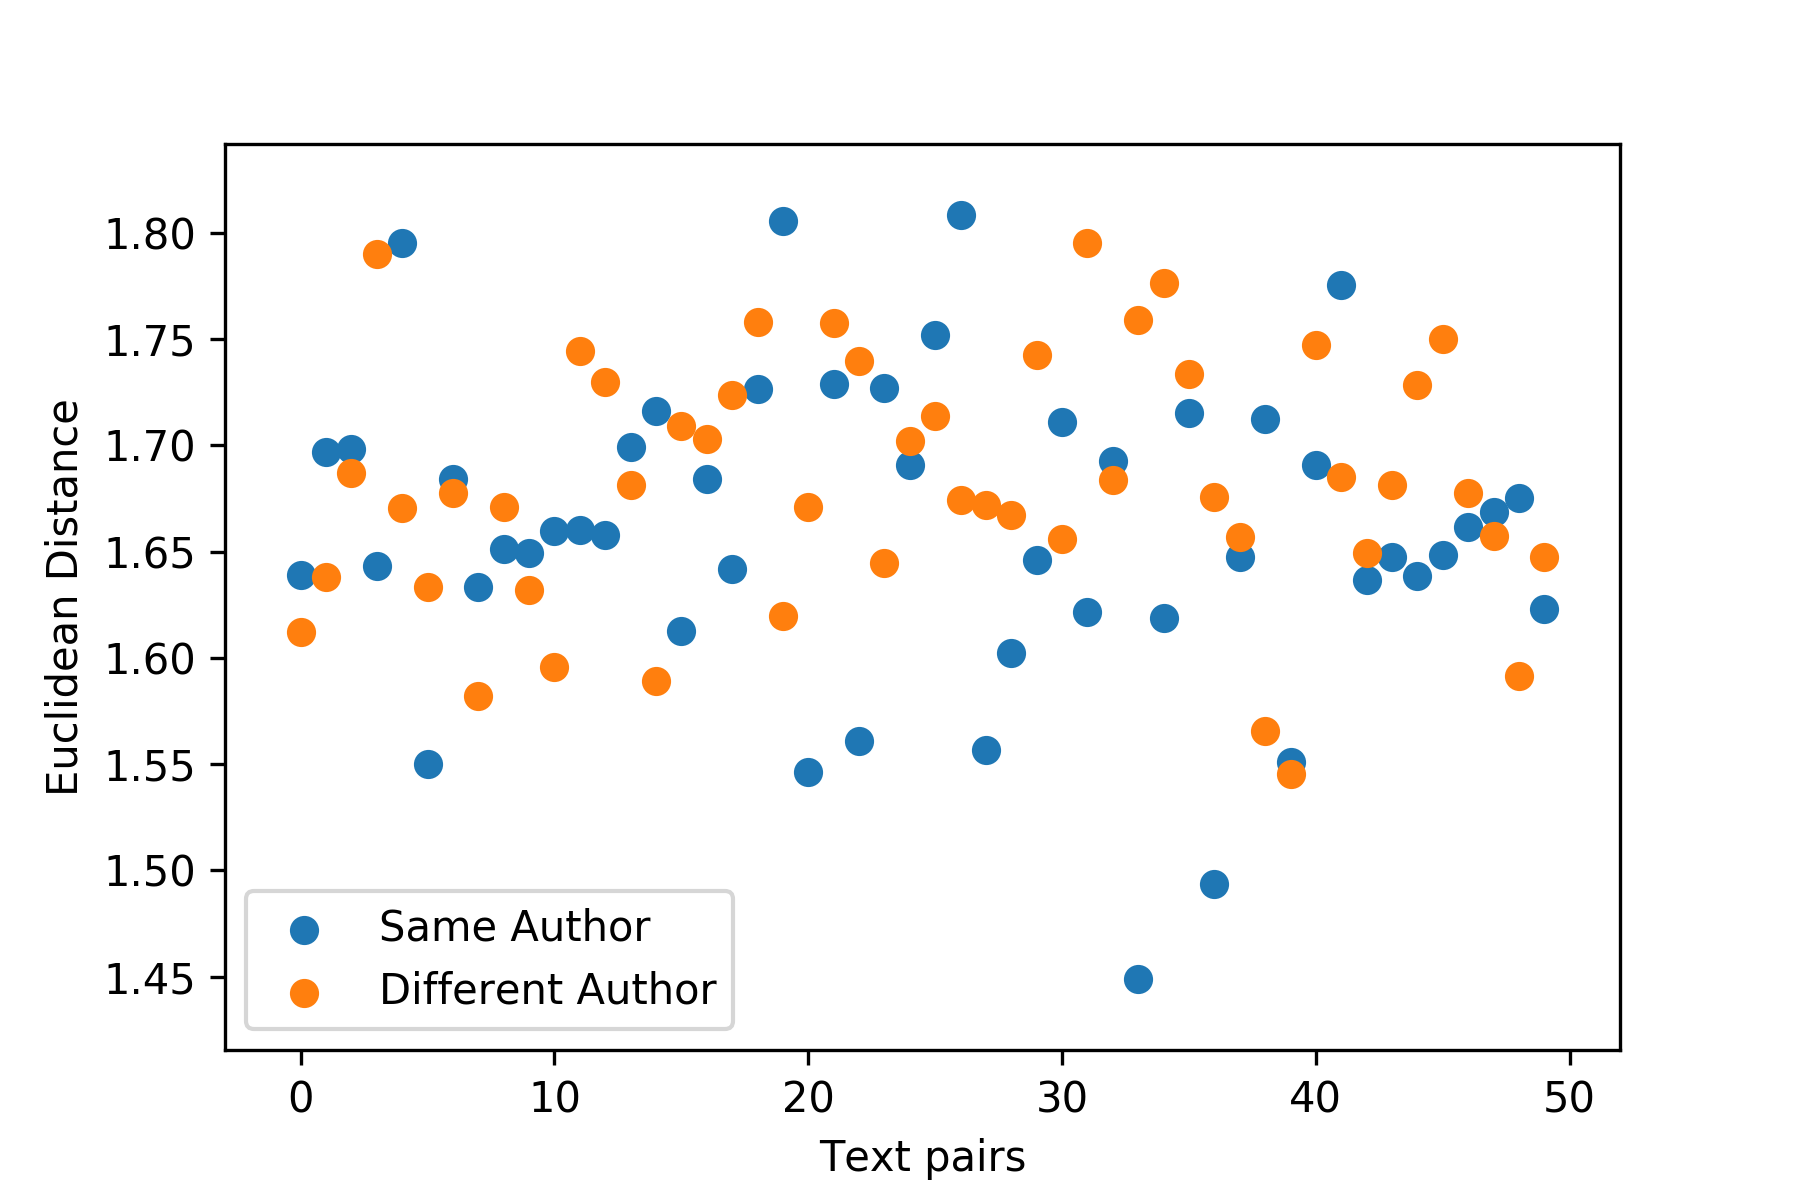
\includegraphics[width=\textwidth]{train_euc}
    \caption{The Euclidean distance between text-pairs for the training set (training on the test set).\label{fig:euc_train}}
  \end{minipage}
  \hfill
  \begin{minipage}[b]{0.49\textwidth}
    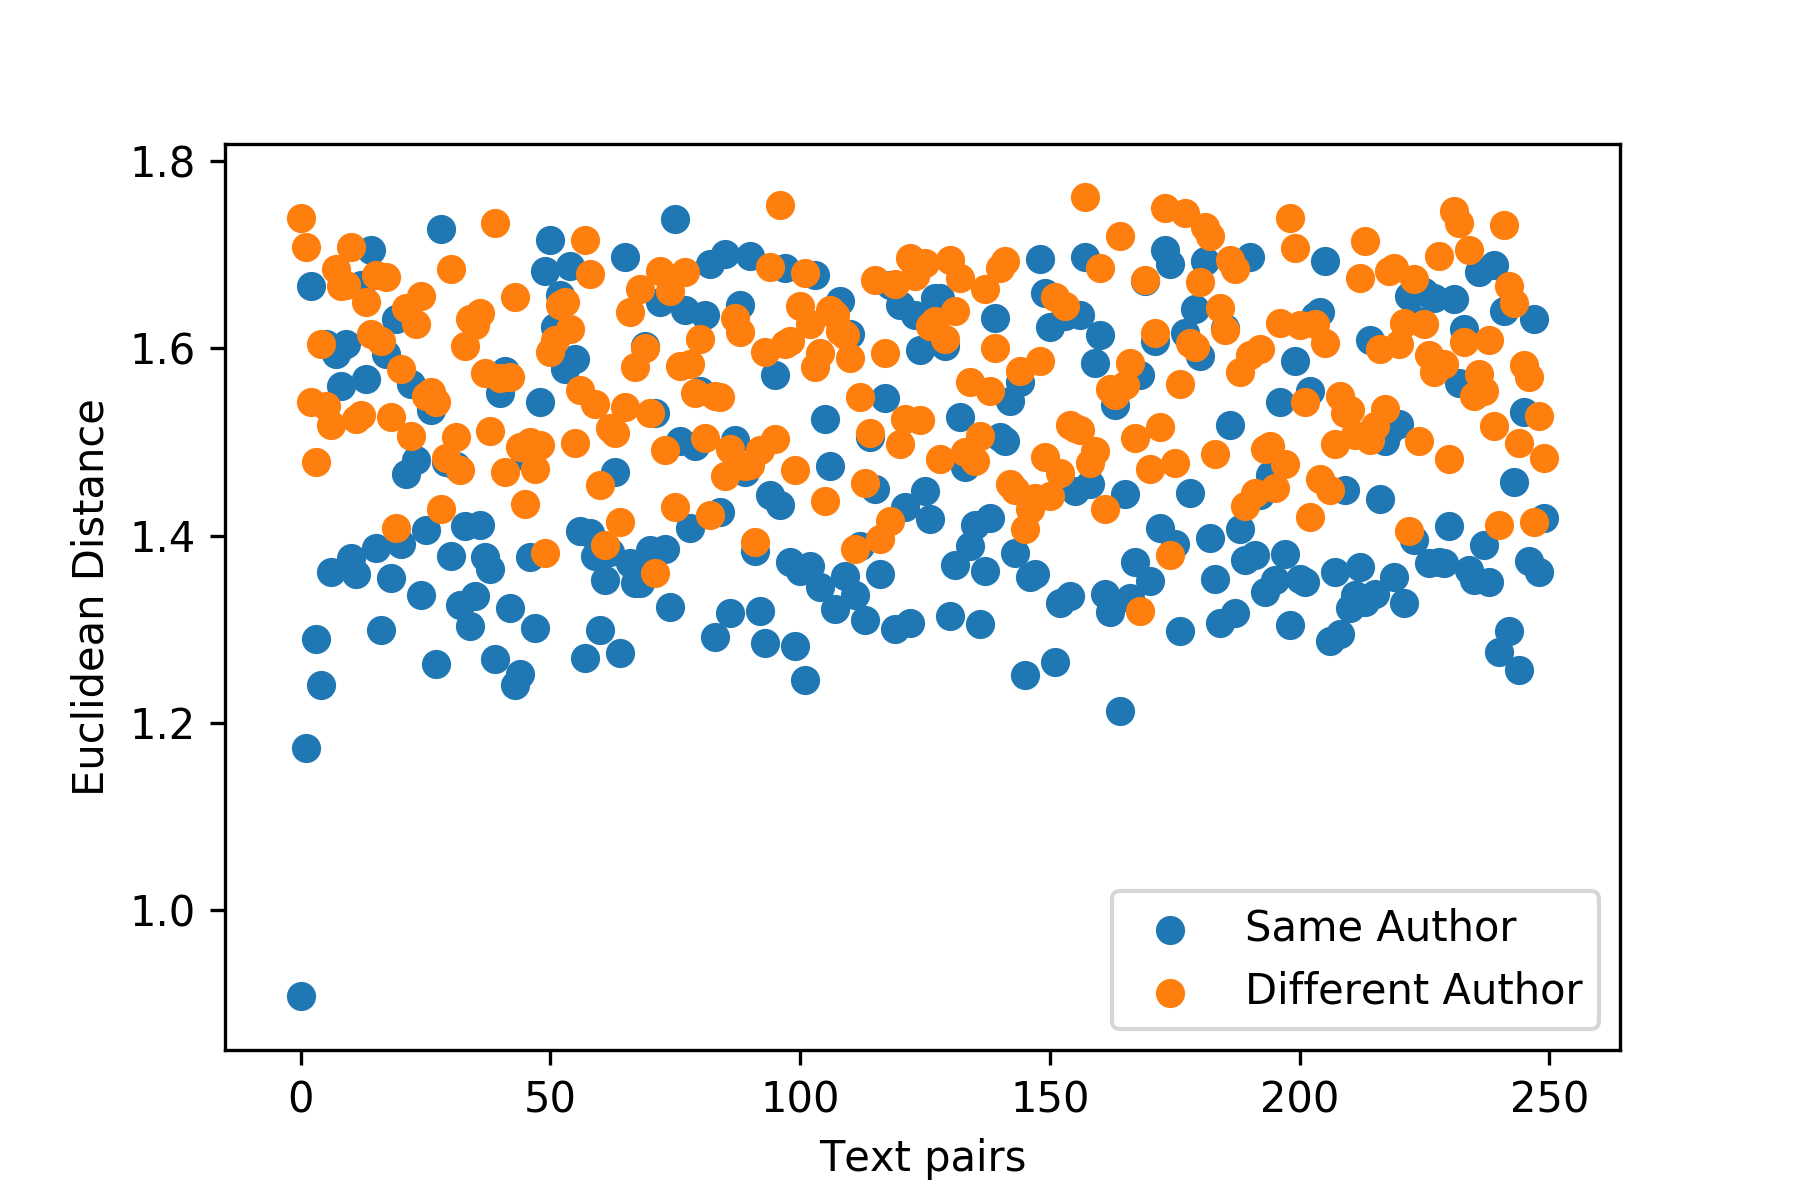
\includegraphics[width=\textwidth]{test_euc}
    \caption{The Euclidean distance between text-pairs for the test set (training on the training set)} \label{fig:euc_test}
  \end{minipage}
  \begin{minipage}[b]{0.49\textwidth}
    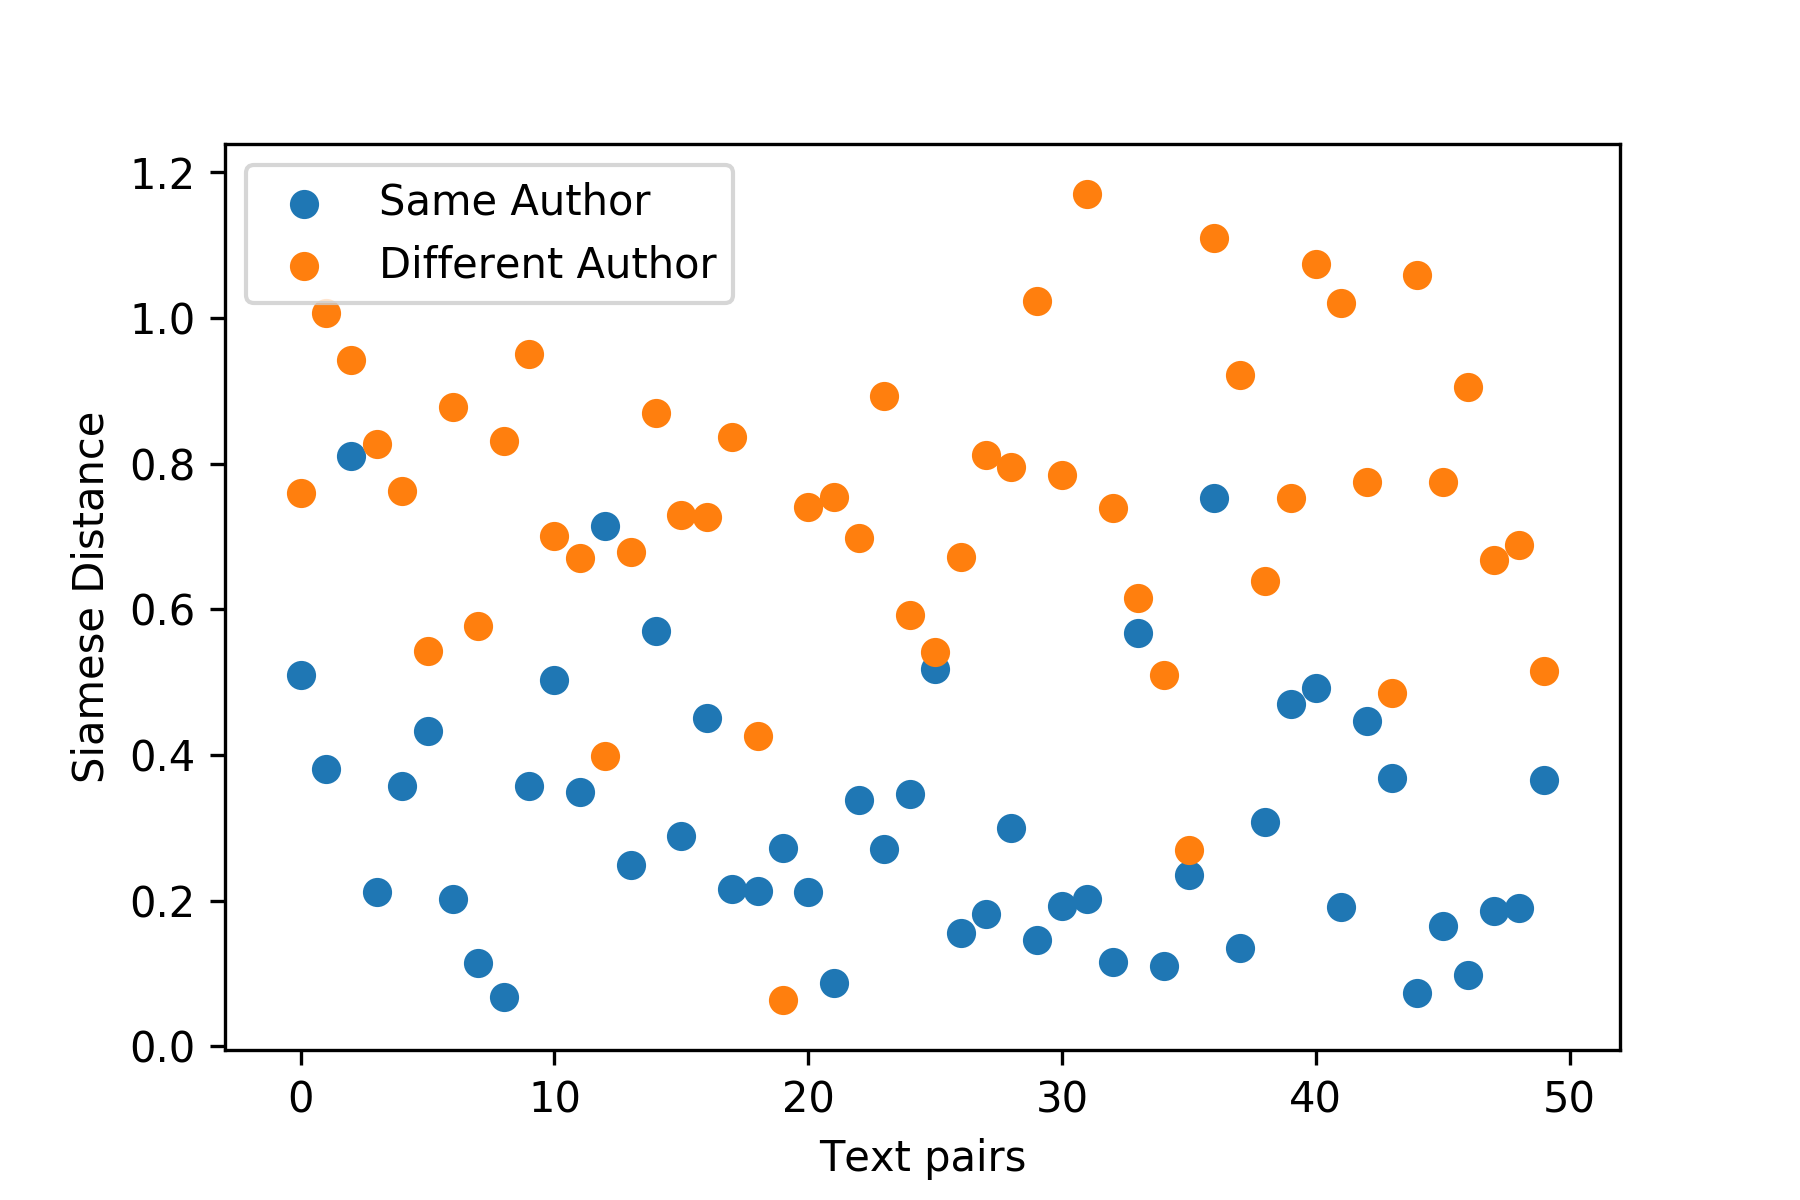
\includegraphics[width=\textwidth]{train_siam}
    \caption{The Siamese learned distance between text-pairs for the training set (training on the test set). \label{fig:siam_train}}
  \end{minipage}
  \hfill
  \begin{minipage}[b]{0.49\textwidth}
    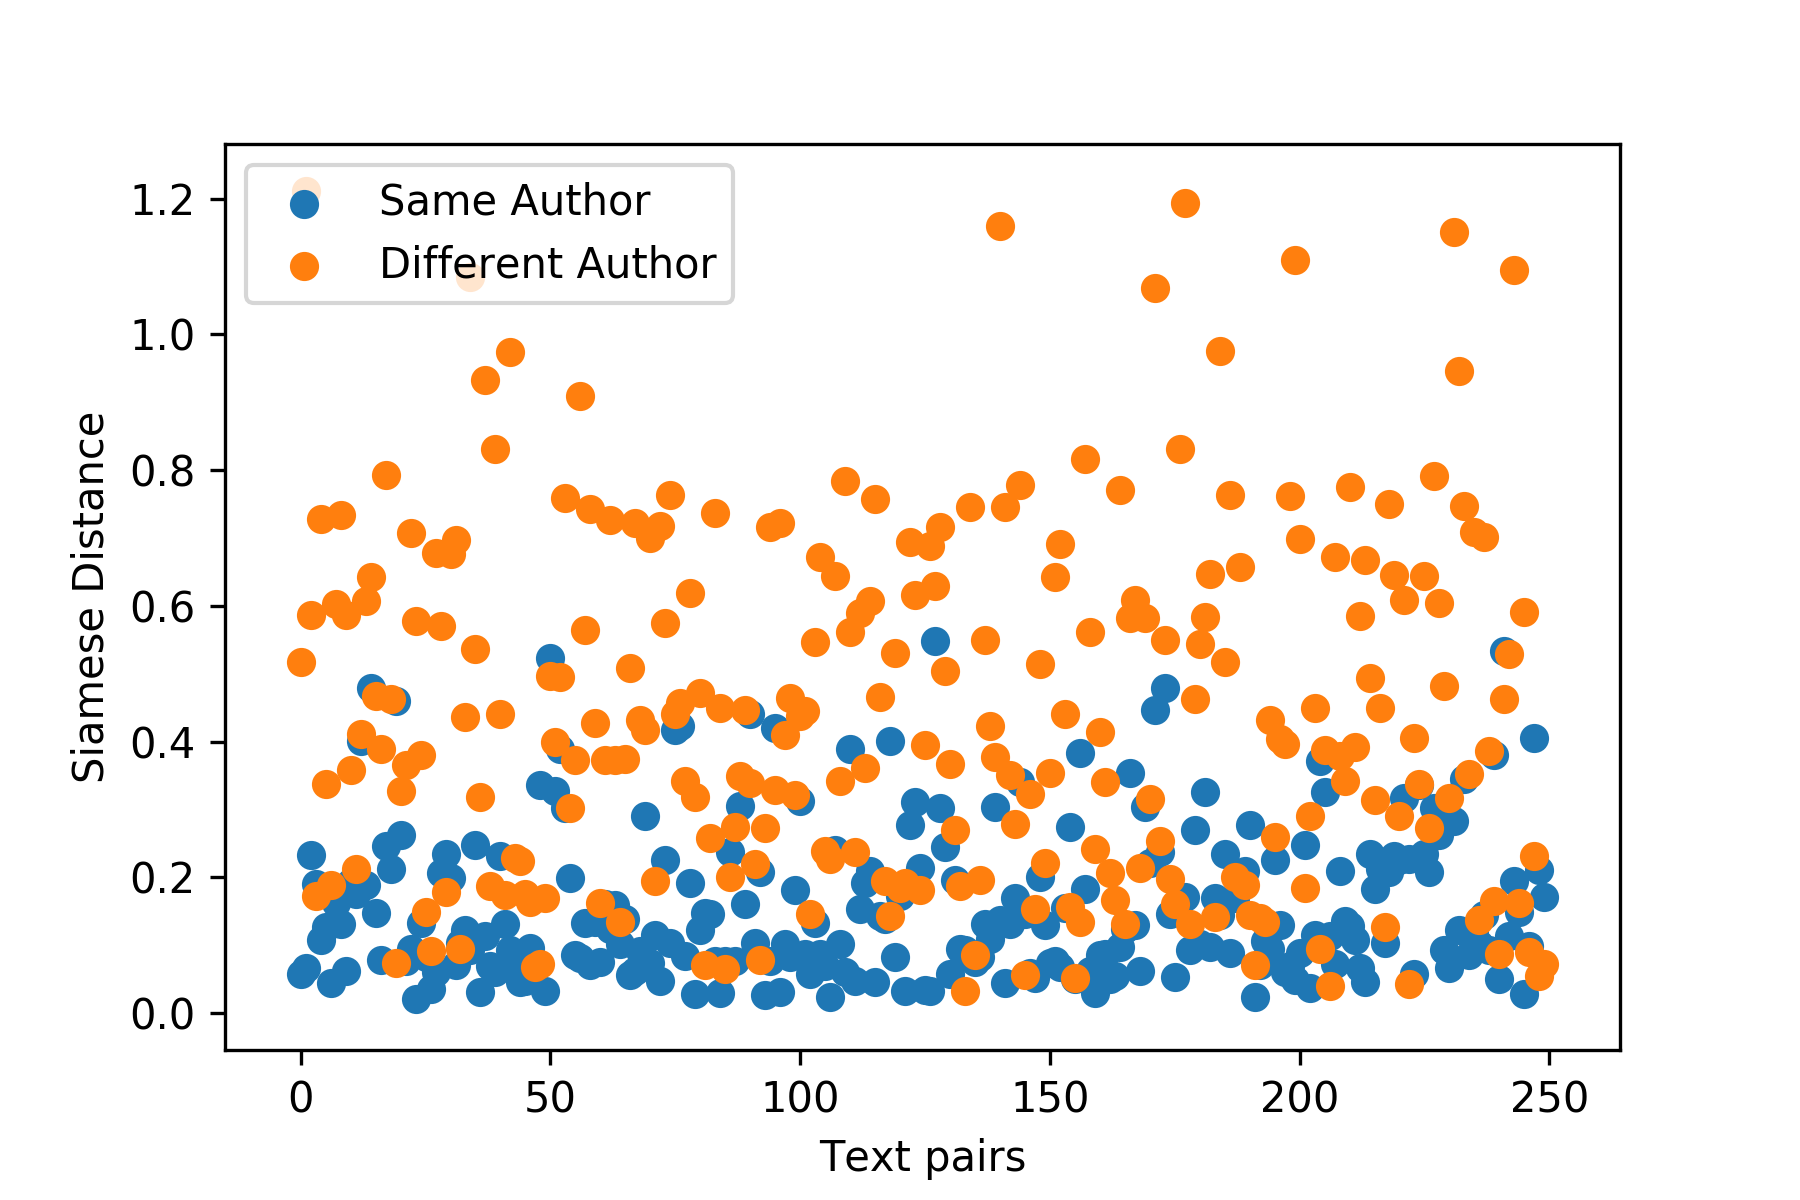
\includegraphics[width=\textwidth]{test_siam}
    \caption{The Siamese learned distance between text-pairs for the test set (training on the training set) \label{fig:siam_test}}
  \end{minipage}
\end{figure}


We present results on the other PAN datasets in Section \ref{res:siamese}.

\chapter{Results}
In this chapter we present the results of the experiments described in Chapter \ref{chap:models}. These results are presented in the same order as we described the methods and models. Where appropriate we compare our results to previous approaches on the same datasets. Note that the results involving the Yelp Dataset were previously presented in our submission to the Yelp Dataset Challenge.\footnote{https://github.com/sixhobbits/yelp-dataset-2017/} 

\section{Unsupervised Statistical Approaches}
\label{res:unsupervised}

\nocite{cappellato2014clef}

For our unsupervised models, we present results on the training and test sets, as these models did not need to be trained. We compare our results to those achieved in the PAN shared tasks. Note that these results are not directly comparable for several reasons. 

First, the systems that were entered for the shared task were designed to work across various languages, while ours focuses on the English parts of the dataset. Second, the PAN participants were aiming to optimize a so-called ``c@1'' metric, in which systems were penalized less for failing to provide a prediction than for providing the wrong one. That is, systems were encouraged to withhold predictions in the case of difficult or borderline text pairs, while our system generated predictions for all instances. Third, the PAN systems aimed to achieve scores as high as possible, while we attempted to build a system that could be easily interpretable and that could help forensic linguists in manual evaluation.

For the PAN 2014 datasets, we compare ourselves to \citet{khonji2014slightly}, 
who achieved the best overall results and the highest accuracy score for the English novels dataset as well as to \citet{frery2014identification} who achieved the best results for English essays. For PAN 2015, we compare ourselves to \citet{bagnall2015author}, who achieved the best results overall and for the English dataset.

\begin{table}[ht]
\caption{\label{tab:unsupres} The comparative results for our Unsupervised method for the basic and correlation models. We present our highest results using thresholds of 0.75 for both models. Khonji=\citet{khonji2014slightly}, Frery=\citet{frery2014identification}, Bagnal=\citet{bagnall2015author}, tr=train, te=test.}
\begin{center}
\begin{tabular}{lrrrrr} 
\toprule
                       &  \bf Ours & \bf Ours correlation & \bf   Khonji & \bf Frery & \bf Bagnall \\
\midrule
\bf 2014 Novels tr     &    0.82    & 0.65     &          &         &       \\
\bf 2014 Novels te     & 0.70       & 0.46     & 0.75     & 0.61   &       \\
\bf 2014 Essays tr     & 0.61       & 0.42     &          &         &       \\
\bf 2014 Essays te     &   0.68     & 0.52     &  0.59    &  0.72  &       \\
\bf 2015 tr            &   0.68     & 0.57     &          &         &       \\
\bf 2015 te            &    0.66    & 0.65     &          &         & 0.81  \\
\bf All data           &    0.56    & 0.57     &          &         &       \\
\bottomrule
\end{tabular}
\end{center}
\end{table}

The full results for the unsupervised models can be seen in Table \ref{tab:unsupres}. Although we did not beat the winners of the PAN shared tasks with our methods, it is interesting that our results are more stable. Of all the systems submitted for PAN 2014, the ones that did well on the English Essays dataset tended to do badly on the English Novels, and vice-versa, whereas our system achieved similar results on both of these datasets. The PAN 2015 test set is a more challenging dataset as it is deliberately chosen to be cross-topic, as discussed before. \citeauthor{bagnall2015author}'s 
high result on this dataset is from a neural network approach that required nearly 22 hours to run, 
while our system runs in a few minutes. 

The effect of the different thresholds on the accuracy score can be seen in Figure \ref{fig:unsupthresh}. We can see that finding the correct threshold is important. Setting the threshold too low results in the system predicting \textit{same-author} for nearly every instance, and setting it to high results in it predicting \textit{different-author} for nearly every instance. An ongoing challenge for Authorship Attribution tasks that rely on a threshold is to find the correct value for this threshold, as in many real-world cases, as previously discussed, there is no dataset similar enough to the questioned works that can be used to train a classifier and find a correct threshold.

\begin{figure}[ht]
    \label{fig:unsupthresh}
    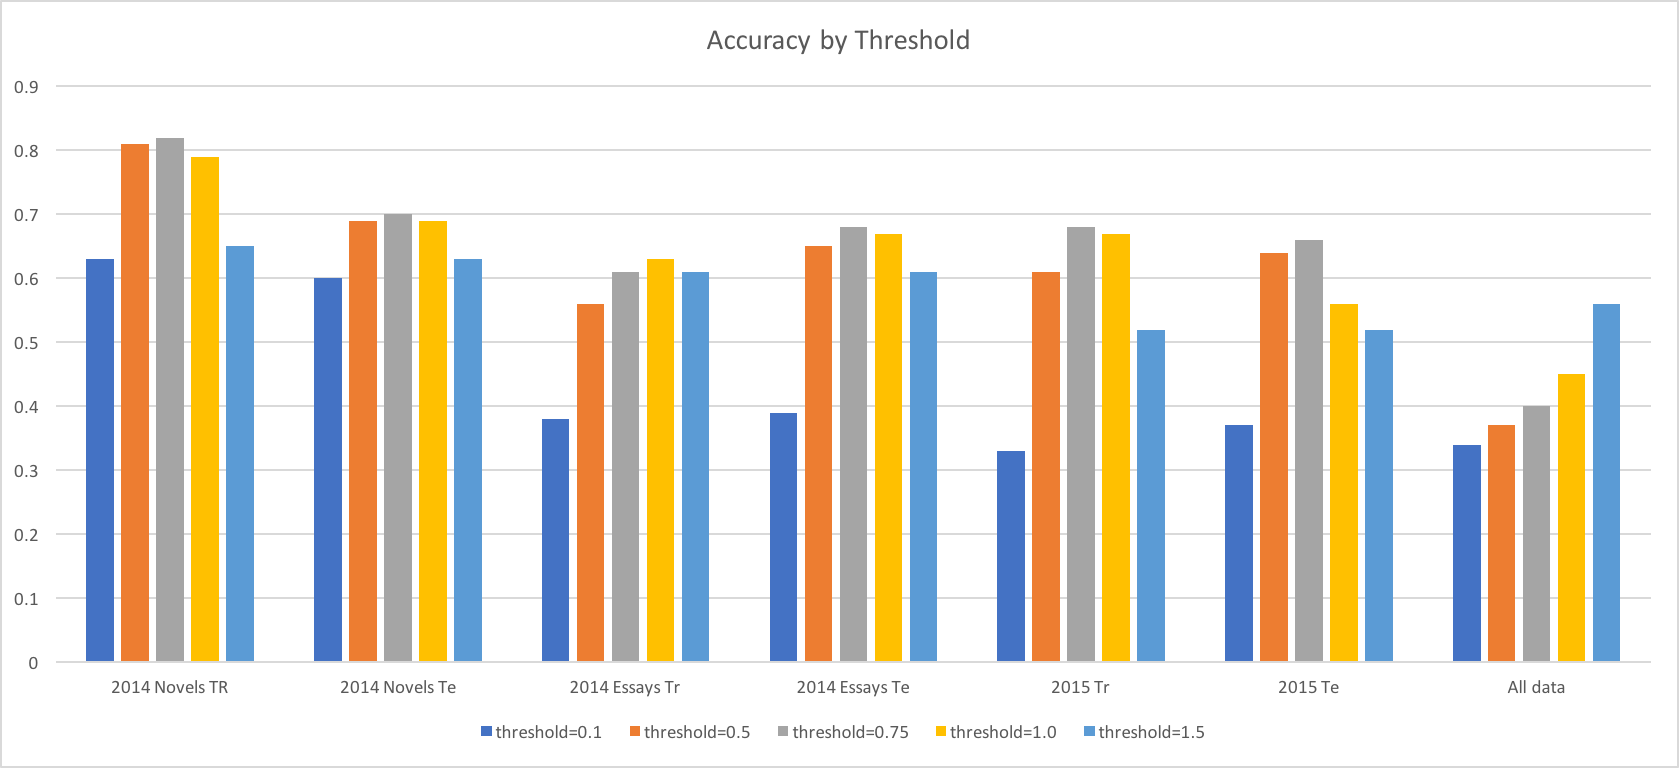
\includegraphics[scale=0.5]{unsupervisedthreshold}
    \caption{The effect of the threshold on the different datasets. Generally setting the threshold too low or too high worsens the results.}
\end{figure}


\section{Support Vector Machine Approaches}
Here we present results for our Support Vector Machine (SVM) approaches for the AID and AV tasks. Unlike the unsupervised approach, the SVM approach did not require language-specific tools, and it scaled well to large datasets. We could therefore test this approach on most of our datasets, but as our Yelp datasets are novel, we cannot compare our results on this dataset to previous attempts.

\subsection{Authorship Identification Tasks}
\label{res:svmaid}
For the AID tasks, we evaluated our models on our Yelp dataset and the C50 dataset. For the former, we have no comparison, as this is the first time that this dataset has been used. However, in Section \ref{res:nn-aid}, we present more discussion about this result when comparing it to our Neural Network model. For the C50 dataset, we compare our results to \citet{houvardas2006ngram}, who introduced the dataset and who presents several results using similar SVM models.

On the Yelp dataset, we achieved an accuracy score of 0.90 using our SVM models. This supports the previous research discussed which showed that Support Vector Machine models are highly effective for many text classification tasks, including Authorship Identification. 

For the C50 dataset, we achieved an accuracy score of 0.72. This is comparable with the work of \citet{houvardas2006ngram}, who reported accuracy scores ranging from 0.69 to 0.74 for various feature selection methods and n-gram ranges.

The fact that we achieved lower scores on the C50 dataset than on the Yelp dataset is interesting because there was more training and test text available in the C50 dataset than the subset of the Yelp dataset that we used. This suggests that authors who write freely on the internet are easier to identify by their writing style than journalists who have been trained to write in similar styles (and who have potentially had their text edited for style by editors and proofreaders). 

\subsection{Authorship Verification Tasks}
\label{res:svmav}

For the Authorship Verification tasks, we achieved the results shown in Table \ref{tab:svmav}.

\begin{table}[ht]
\caption{\label{tab:svmav} The comparative results for our Support Vector Machine models. We present accuracy scores alongside our F1 scores in order to be able to compare to previous high scores at PAN. \textit{B/K} is \citet{bagnall2015author} for 2015 datasets and \citet{khonji2014slightly} for 2014 datasets. ``Yelp short'' and ``Yelp long'' refer to the datasets summarized in Table \ref{verdata-table}}.
\begin{center}
\begin{tabular}{lrrr} 
\toprule
                       &  \bf F1 &    \bf Acc & \bf B/K Acc. \\
\midrule
\bf 2014 en Novels tr     &   0.72     & 0.72   &          \\
\bf 2014 en Novels te     &   0.63     & 0.64   &   0.75    \\
\bf 2014 en Essays tr     &   0.61     & 0.61   &           \\
\bf 2014 en Essays te     &   0.58     & 0.58   &   0.59   \\
\bf 2014 nl Reviews tr     &   0.62    & 0.62  &           \\
\bf 2014 nl Reviews te     &   0.38    & 0.52  &    0.74   \\
\bf 2014 nl Essays tr     &   0.69     & 0.68  &           \\
\bf 2014 nl Essays te     &   0.66     & 0.65  &   0.91    \\
\bf 2014 gr tr             &   0.50    & 0.52  &           \\
\bf 2014 gr te             &   0.47    & 0.51  &   0.89    \\
\bf 2014 es tr             &   0.62    & 0.64  &           \\
\bf 2014 es te             &   0.67    & 0.69  &      0.90 \\
\bf 2015 en tr             &   0.82    & 0.82  &         \\
\bf 2015 en te             &   0.58    & 0.61  &    0.81 \\
\bf 2015 nl tr             &   0.71    & 0.71  &         \\
\bf 2015 nl te             &   0.64    & 0.64  &   0.70  \\
\bf 2015 gr tr             &   0.56    & 0.59  &         \\
\bf 2015 gr te             &   0.57    & 0.57  &    0.88 \\
\bf 2015 es tr             &   0.59    & 0.61  &         \\
\bf 2015 es te             &   0.33    & 0.50  &    0.89 \\
\bf Yelp short             &           & 0.92  &         \\
\bf Yelp long              &           & 0.95  &         \\ 
\hline
\end{tabular}
\end{center}
\end{table}

For the PAN datasets, we failed to achieve higher scores than those achieved by previous PAN winners. However, our method achieved above baseline results for nearly all subsets of PAN and required no tuning or modification for the different datasets. It was also substantially more efficient than the winning PAN models, requiring only a few minutes to run instead of the run times of more than a day reported by the top PAN participants \cite{stamatatos2015overview}.

For the Yelp datasets, we can see that shorter texts are more difficult to accurately classify, even though we had more examples to train on (71\,300 and 38\,900 respectively). However, in both cases our novel approach achieved very high results. As discussed before, these results are especially interesting as the authors in the test set are disjoint from those in the training set (in fact, no author is represented more than once). It is impressive that even using a simple approach, a supervised classifier is able to make meaningful decisions about authors that it has not seen examples of during the training phase.

Although we still need a fair amount of text for each known author, this is far less than what is needed to achieve reasonable results in an identification task. As mentioned before, the verification task can be used a stepping-stone to solve many other authorship attribution tasks, including identification. We could, for example, do pairwise comparisons across all reviews in a corpus to find the likelihood of a single author using multiple accounts, or do a pairwise comparison of all the reviews associated with a single username to find out if it is likely that more than one person uses that account.


\section{Neural Network Approaches}
In this section we present our results on the AID tasks and AV tasks for our Neural Network models. First we present our results on the AID tasks using our character-level language models. This is followed by our results on the AV tasks using Siamese Neural Network models.

\subsection{Authorship Identification Tasks}
\label{res:nn-aid}
This was the most computationally expensive part of our work, as we needed to train an author-specific language model for each candidate author, and then evaluate each test text against each language model. To train and evaluate the models in a reasonalbe amount of time, we used a cloud machine with four virtual CPUs, 61 GiB of RAM and an NVIDIA K80 GPU with 2 496 parallel processing cores and 12 GiB of GPU memory. Even with this extra compute capacity, this experiment took approximately 15 hours to run, substantially longer than our other experiments. Due to time and computate capacity limitations, we therefore present results only against a single dataset, namely the Yelp dataset that we introduced as part of our work.

We achieved an accuracy score of 0.90 on the Yelp dataset. As this is the first time that this dataset has been used for Authorship Identification, we cannot present any comparitive results to previous attempts or models. However, this was the same score achieved by our SVM model, described above, suggesting that character-level neural language modelling can provide an effective solution to at least some Authorship Attribution tasks, which supports the assertions of \citet{bagnall2015author}. 

\subsection{Authorship Verification Tasks}
\label{res:siamese}

We experimented with our Siamese model using all of the PAN 2014 and PAN 2015 data, across various languages. Because results from this model varied substantially between runs, we present average F1-scores over 10 runs, (where we average the F1 score of the positive and negative classes for each run, and then average this over all runs),
along with the lowest and highest score achieved. We further present averaged accuracies over 10 runs in order to compare to previous PAN results for which F1 scores are not available.

\begin{table}[ht]
\caption{\label{tab:siameseres} The comparative results for our Siamese method, averaged over 10 runs. We present accuracy scores alongside our F1 scores in order to be able to compare to previous high scores at PAN. \textit{B/K} is \citet{bagnall2015author} for 2015 datasets and \citet{khonji2014slightly} for 2014 datasets. Note that datasets marked with * were used to tune the models and the results should not be taken as indicative of evaluation.}
\begin{center}
\begin{tabular}{lrrrrr} 
\toprule
                       &  \bf Avg F1 & \bf Min F1 & \bf Max F1 & \bf Avg Acc & \bf B/K Acc. \\
\midrule
\bf 2014 en Novels tr     &   0.64    & 0.54         & 0.70      & 0.66   &          \\
\bf 2014 en Novels te     &   0.59        & 0.52     & 0.61     & 0.64   &   0.75    \\
\bf 2014 en Essays tr     &   0.49       & 0.44      & 0.57     & 0.51   &           \\
\bf 2014 en Essays te     &   0.50     & 0.35        &  0.60    & 0.54   &   0.59   \\
\bf 2014 nl Reviews tr     &   0.34     & 0.33        &  0.38   & 0.50  &           \\
\bf 2014 nl Reviews te     &   0.36     & 0.33        &  0.40    & 0.51  &    0.74   \\
\bf 2014 nl Essays tr     &   0.65     & 0.52        &  0.78    & 0.69  &           \\
\bf 2014 nl Essays te     &   0.59     & 0.50        &  0.69    & 0.64  &   0.91    \\
\bf 2014 gr tr             &   0.40     & 0.33        &  0.49   & 0.53  &           \\
\bf 2014 gr te             &   0.33     & 0.33        &  0.33   & 0.50  &   0.89    \\
\bf 2014 es tr             &   0.46     & 0.42        &  0.49   & 0.53  &           \\
\bf 2014 es te             &   0.40     & 0.37        &  0.44   & 0.53  &      0.90 \\
\bf 2015 en tr*             &   0.82     & 0.76        &  0.91    &  0.82  &         \\
\bf 2015 en te*             &   0.66     & 0.57        &  0.74    &  0.68  &    0.81 \\
\bf 2015 nl tr             &   0.46     & 0.33        &  0.57    &  0.54  &         \\
\bf 2015 nl te             &   0.45     & 0.37        &  0.50    &  0.50  &   0.70  \\
\bf 2015 gr tr             &   0.48     & 0.37        &  0.55    &  0.53  &         \\
\bf 2015 gr te             &   0.35     & 0.33        &  0.37    &  0.50  &    0.88 \\
\bf 2015 es tr             &   0.59     & 0.51        &  0.70    &  0.61  &         \\
\bf 2015 es te             &   0.56     & 0.49        &  0.64    &  0.62  &    0.89 \\
\bottomrule
\end{tabular}
\end{center}
\end{table}

The results are presented in Table \ref{tab:siameseres}, where we can see that the Siamese model did not perform well, underperforming previous PAN winners and in some cases failing to outperform a random baseline. Closer examination of the very low results showed that in these cases the Siamese Network failed to learn anything meaningful from the training dataset, and always or almost always predicted the same label for all test instances. 

We find it interesting that the results for the Siamese Neural Network varied substantially between runs. This could raise some concerns over previous PAN results, in which only a single run was carried out. 
Specifically, the best-performing system in 2014 took over 20 hours to run, and in 2015 the best-performing system needed more than 50 hours to run on the test dataset. This makes it more difficult to test these systems thoroughly over multiple runs.

Overall, we are disappointed that our Siamese Model did not perform better, as believed that this model was the best theoretical fit for task. We are still hopefull that with more experimentation with network architecture, preprocessing, and different datasets that Siamese Models might prove more practically suitable to the AV task.


\chapter{Conclusion}

In this chapter, we provide a brief summary and discussion of our methods and results, suggesting areas for future work where applicable.

We presented several methods for identifying authors by their writing style alone. Although our results were in many cases lower than we hoped, we believe that all three broad techniques that we presented (namely, unsupervised statistical approaches; approaches using Support Vector Machines; and approaches using Neural Networks) provide value in different ways. We discuss each of these below.

Our Unsupervised approach used descriptive statistics to compare texts of interest to larger corpora. If two texts differ from the corpus in the same, this provides evidence that both texts are written by the same author. This method is interesting in that it is not a ``black box'', unlike the other methods. This means that it can provide expert humans with interpretable data, and can be used in combination with manual analysis or with the other methods to provide evidence about who the author of a disputed work is. This is the method that is easiest to understand, and can therefore be used to provide evidence and arguments to non-experts, for example, in a court of law. Although the results we achieved with this method were not brilliant, we believe that the ease of interpretation is important in many cases. More research is needed to find features and data that lead to better and more consistent results. Further, this technique relies on many language-specific tools, and would face large limitations if used for smaller languages for which such tools are often not available.

Our Support Vector Machine approaches are valuable for their simplicity and scalability. They were able to quickly process large amounts of data, making them practical for large datasets that would take far too long to process using our neural network methods, or many methods presented by other researchers that could achieve state-of-the-art results on smaller datasets. These models also showed flexibility, and were able to work across datasets, languages, and tasks. More research is needed to find out how to select the right training data to make these models perform well in practical situations where the the test data is unique.

The Neural Network methods we presented arguably have the most potential. With so many variations in model architecture and hyperparameters to explore, they are also the most difficult to get right. We expect many advances in the near future in using Neural Networks for NLP tasks, and we expect that some of these advances will be useful to finding a Neural Network configuration that is able to accurately model writing style. More work is needed to experiment with the almost countless ways to solve Authorship Attribution tasks.
\label{chap:con}


% \input{Chap1.tex}
%\input{Chap2.tex}

\bibliographystyle{ruauthordate}    % authordate style 
 
\bibliography{ref}   	% load in the info produced from ref.bib 

\end{document}

